\SetPicSubDir{ch-Iconnotif}
\SetExpSubDir{ch-Iconnotif}

\chapter{Noticon: Reducing distractions from OHMD notifications through icon augmentation}
\chaptermark{Noticon}
\label{ch:Iconnotif}


\section{Chapter overview}

This chapter explores the use of pattern perception abilities to present OHMD notifications. To answer the high-level RQ (\autoref{sec:Intro:thesis_RQ}), \RQMainIconNotif{}, we selected pictograms to support pattern perception and to concretize the notification design, focusing specifically on calendar notifications within a work setting (\autoref{sec:IconNotif:overview:goals}). Furthermore, this question was divided into design and evaluation aspects:
\begin{enumerate}
    \item How can we convert calendar notification content into a pictogram format?
    \item How effective is such a pictogram format in reducing attention costs associated with calendar notifications?
\end{enumerate}

To address the first sub-question, we transformed text-only notifications into \iconnotif{s} (i.e., notifications with content partially represented by pictograms, such as icons) based on the perceptual property that shapes are easier to identify than text.

To address the second sub-question, we compared \textnotif{s} with \iconnotif{s} in a context less explored in prior work (\autoref{sec:Relatedwork:pattern_perception}) — as OHMD notifications — in four studies (three controlled, one realistic) to understand the factors influencing the effective use of pictograms. Our results suggested that transforming \textnotif{s} into \iconnotif{s} could reduce distractions and improve multitasking performance without compromising the noticeability or understandability of notifications. However, the effectiveness of \iconnotif{} depends on icon familiarity, \encodingcomplexity{}, notification conciseness, and environmental brightness. We concluded that carefully designed \iconnotif{s} can offer an appealing and less distracting notification format for OHMDs. Lastly, we discussed guidelines for transforming \textnotif{s} into their \iconformat{} and examined plausible explanations for the observed disparity in literature.

This chapter contains adapted materials (including figures and tables) from our publication reporting on our work and studies conducted \cite{janaka_can_2023}.







\section{Introduction}
\label{sec:Iconnotif:introduction}

As established in \autoref{ch:Relatedwork}, more attention control is required in certain work settings, and distractions from OHMD notifications should be minimized accordingly. One strategy to mitigate such disruption involves presenting notifications as pictograms instead of text. Pictogram-based notifications have previously been explored within desktop computing \cite{warnock_multiple_2013, warnock_subjective_2011, somervell_evaluating_2002}, navigational \cite{ells_rapid_1979, camacho_icons_1990, houts_role_2006}, and healthcare \cite{houts_role_2006, leos_toro_perceptions_2019} contexts, though the efficacy results have been inconsistent (\autoref{sec:Relatedwork:pattern_perception}).

This chapter examines the use of pictograms in OHMD notifications and the factors affecting their efficacy. From a series of four studies (three laboratory-based and one realistic), we found that the effectiveness of pictogram notifications depends on several factors, including an individual's familiarity with the icon (i.e., frequency of use and intuitiveness of the depicted object \cite{isherwood_icon_2007}), the \encodingcomplexity{} (i.e., the amount of textual information encoded by the icon), and the environmental context. These crucial factors allow for a more comprehensive evaluation of the benefits of pictograms over text notifications.

Our results suggest potential scenarios and design guidelines for using \iconnotif{s} within the heads-up computing paradigm. We recommend \iconnotif{s} for everyday short notifications such as reminders and todos, as they lessen the impact of notification interruption while supporting information needs. Moreover, establishing a standard icon set for OHMD notifications could enhance the advantages of the \iconformat{}.

The contributions of this chapter are threefold: 1) a revisitation of the factors affecting the effectiveness of pictogram notifications in OHMDs within multitasking contexts; 2) an enhanced understanding of how text and pictogram formats used for OHMD notifications differ in terms of interruption, reaction, and comprehension (IRC framework); and 3) an evaluation of the generalizability of results yielded in lab settings to realistic settings, based on which we discuss the trade-offs and insights of using text and \iconnotif{s}.











\section{\Iconnotif{s} on OHMDs}
\label{sec:Iconnotif:icon_augmentation}

As we examine the differences between pictograms and text, we base our investigation on a practical HCI problem: designing effective notifications on OHMDs for multitasking usage. Specifically, we're interested in whether integrating \textit{icons} into OHMD notifications can minimize attention costs (e.g., distraction, task interference). While current mobile notifications use icons to display the source of the notification (e.g., app, sender) as a supplement, the content of the notification is still entirely presented in a text format (e.g., \autoref{fig:IconNotif:overview:android_notification_ori}) \cite{apple_notifications_2022, android_android_2021}. Contrarily, our work investigates how to partially represent the content of the notifications themselves via icons (e.g., \autoref{fig:IconNotif:overview:android_notification_proposed}), a significant departure from existing approaches.

Icons are symbolic representations of objects and concepts and are widely used visual elements in user interfaces and traffic signs \cite{tijus_design_2007, caplin_2001_icon}. Being graphical, icons are easier to recognize and remember \cite[Ch~6]{tijus_design_2007, wickens_engineering_2015}. However, unlike pictures--- which can lead to a wide range of interpretations \cite{theios_theoretical_1989}--- each icon is typically designed to represent a single meaning \cite{caplin_2001_icon}. In this sense, it is functionally similar to logographical words (e.g., Chinese characters). A recent study conducted by Huang et al. \cite{huang_how_2015} using brain imaging has shown that icons are not processed cognitively as logographical words (although both stimulate the brain's semantic system needed for language processing) but are more akin to images and pictures. Therefore, icons can leverage our brain's unique capabilities to process images. Icons can be used either alone or in combination with text. From previous research, we learned that icons alone could be difficult to interpret \cite{wiedenbeck_use_1999}, so we decided to combine icons with text to create \iconnotif{s} and examine whether this particular form of notifications offers any advantages over text alone.




\subsection{\Iconnotif{} design}

Given the multitude of notification types, we chose to focus on calendar notifications for this investigation due to their high frequency in daily life ($M \approx{} 4,\: SD > 16$ notifications per day according to Table~2 in \cite{sahami_shirazi_large_scale_2014}), uniform structure (\autoref{sec:IconNotif:overview:notification_design}), and high perceived value \cite{tungare_exploratory_2008, kelley_how_1982, sahami_shirazi_large_scale_2014}.



\subsubsection*{Notification structure}
\label{sec:IconNotif:overview:notification_design}

Calendar notifications can be thought of as comprising two parts: 1) primary information (e.g., event/action), and 2) secondary information (e.g., time, person, or location). The notification "Meeting in 30 minutes" can be decomposed into "<\primaryinfo{}: meeting, \secondaryinfo{}: 30 minutes>". To convert the text notification into an \iconnotif{}, \primaryinfo{} is represented using icons, while \secondaryinfo{} is represented using numbers or text. An example is shown in \autoref{fig:IconNotif:overview:notification_mapping}.
For brevity, prepositions, such as the word 'in' from the notification "Meeting in 30 minutes", were removed, and abbreviations were used in the \iconnotif{}, as our pilot studies have shown that they do not impact comprehension.

\begin{figure*}[hptb]
  \centering
\begin{subfigure}{.5\linewidth}
  \centering
  
\includegraphics[width=0.9\linewidth]{\Pic{overview/android_notif_ori.jpg}}
  \caption{}
  \label{fig:IconNotif:overview:android_notification_ori}	  
\end{subfigure}%
\begin{subfigure}{.5\linewidth}
  \centering
  
\includegraphics[width=0.9\linewidth]{\Pic{overview/android_notif_proposed.jpg}}
  \caption{}
  \label{fig:IconNotif:overview:android_notification_proposed}	  
\end{subfigure}

\begin{subfigure}{1\linewidth}
  \centering
  \scalebox{0.87}{
    \begin{tabular}{@{}llll@{}}
    \toprule
    regular \textnotif{}                            & \textless{}\primaryinfo{}, \secondaryinfo{}\textgreater{}                                 & \multicolumn{2}{l}{\iconnotif{}} \\ \midrule
    Meeting at 4 pm                 & \textless{}meeting, 4 pm\textgreater{}      &    
\includegraphics[width=6mm]{\Pic{icons/img_meeting4.png}}       & \hspace{1mm} 4 pm          \\
    
    Doctor's appointment in 2 hours & \textless{}doctor appointment, 2 hrs\textgreater{} &    
\includegraphics[width=6mm]{\Pic{icons/img_doctor4.png}}       & \hspace{1mm} 2 hrs         \\ \bottomrule
    \end{tabular}
    }
\caption{}
    \label{fig:IconNotif:overview:notification_mapping}	  
\end{subfigure}
  \caption[A comparison between \textnotif{s} and \iconnotif{s}]{A comparison between \textnotif{s} and \iconnotif{s}. (a) A typical calendar notification \cite{android_android_2021, apple_notifications_2022} where the content is fully represented by text.  (b) The proposed \iconnotif{} where the content is partially represented via icons. (c)} Examples of \textnotif{} to \iconnotif{} mapping. Icon source: \flatIcons{}.
  \label{fig:IconNotif:overview:text_vs_icon_notifications}	
\end{figure*}




\subsubsection*{Icon selection and design calibration}
\label{sec:IconNotif:overview:icon_notif_design}

To minimize the familiarity gap, we selected widely used icons from \materialIcons{}\footnote{Material design icons - \url{https://material.io/resources/icons/?style=outline}} and \flatIcons{}\footnote{Flaticon website - \url{https://www.flaticon.com/}}. We chose the outline style, as it has been demonstrated that on OHMDs, this style is preferable since it allows for better environmental awareness, enhancing multitasking performance \cite{ram_lsvp_2021}.

To ensure a fair comparison, a designer, a researcher, and a proofreader independently evaluated the \textnotif{s} and their corresponding \iconnotif{s} for similarity in informational content and intuitiveness. Twenty-four calendar notifications, adapted from real notifications, were designed in \textnotif{} and corresponding \iconnotif{} sets (e.g., \autoref{fig:IconNotif:overview:notification_mapping}) through two iterations until raters reached full consensus. See \autoref{tab:IconNotif:study1:calendar_notification} for details.


\begin{table}[hptb]
  \centering
  \caption[Calendar notifications used in \studyone{}]{Twenty-four calendar notifications used in \studyone{} with their \textformat{} and \iconformat{}. These are adapted from real mobile-phone notifications. Icon sources: \materialIcons{}  and \flatIcons{}. Each icon's source is attached as a hyperlink to the icon itself.}
  \small
  \label{tab:IconNotif:study1:calendar_notification}
    \begin{tabular}{@{}p{5.5cm}p{1cm}p{1.8cm}@{}}
    \toprule
    \textformat{}                            & \multicolumn{2}{l}{\iconformat{}} \\ \midrule
    
    Meeting at 4 pm                 &   
\includegraphics[height=6mm]{\Pic{icons/img_meeting4.png}}       & \hspace{1mm} 4 pm          \\    
    
    Doctor's appointment in 2 hours &  
\includegraphics[height=6mm]{\Pic{icons/img_doctor4.png}}       & \hspace{1mm} 2 hrs         \\ 

    Lunch with Lee                 &   
\includegraphics[height=6mm]{\Pic{icons/img_lunch4.png}}       & \hspace{1mm} Lee          \\  

    Birthday party tomorrow                 &   
\includegraphics[height=6mm]{\Pic{icons/img_birthday4.png}}       & \hspace{1mm} 1 d          \\  

    Visitor coming on Friday                 &   
\includegraphics[height=6mm]{\Pic{icons/img_visitor4.png}}       & \hspace{1mm} Friday          \\  

    Car is arriving in 5 minutes                 &   
\includegraphics[height=6mm]{\Pic{icons/img_car4.png}}       & \hspace{1mm} 5 min          \\  

    Email meeting agenda                 &   
\includegraphics[height=6mm]{\Pic{icons/img_email4.png}}       & \hspace{1mm} agenda          \\  

    Delivery in 3 days                 &   
\includegraphics[height=6mm]{\Pic{icons/img_delivery4.png}}       & \hspace{1mm} 3 d          \\  

    Pay \$100                 &   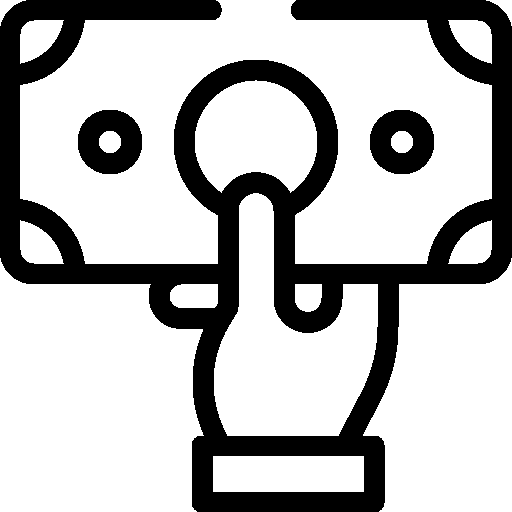
\includegraphics[height=6mm]{\Pic{icons/img_pay_cash4.png}}       & \hspace{1mm} \$100          \\  

    Credit card bill today                 &   
\includegraphics[height=6mm]{\Pic{icons/img_credit_card4.png}}       & \hspace{1mm} today          \\  

    Presentation at noon                 &   
\includegraphics[height=6mm]{\Pic{icons/img_presentation2.png}}       & \hspace{1mm} 12 pm          \\  

    Pay rental on Monday                 &   
\includegraphics[height=6mm]{\Pic{icons/img_pay_rent4.png}}       & \hspace{1mm} Monday          \\  
    \bottomrule
    \end{tabular}\quad %
    \begin{tabular}{@{}p{5.5cm}p{1cm}p{1.8cm}@{}}
    \toprule
    \textformat{}                            & \multicolumn{2}{l}{\iconformat{}} \\ \midrule
    
     Buy milk and eggs tonight                 &   
\includegraphics[height=6mm]{\Pic{icons/img_milk_eggs4.png}}       & \hspace{1mm} tonight          \\  

    Exercise in 40 minutes                 &   
\includegraphics[height=6mm]{\Pic{icons/img_exercise4.png}}       & \hspace{1mm} 40 min          \\  

    Check flight status                 &   
\includegraphics[height=6mm]{\Pic{icons/img_flight4.png}}       & \hspace{1mm} status          \\  

    Reply Alex                 &   
\includegraphics[height=6mm]{\Pic{icons/img_reply4.png}}       & \hspace{1mm} Alex          \\  

    Coffee break at 3 pm                &   
\includegraphics[height=6mm]{\Pic{icons/img_coffee4.png}}       & \hspace{1mm} 3 pm          \\  
    
    Renew driving license                 &   
\includegraphics[height=6mm]{\Pic{icons/img_license4.png}}       & \hspace{1mm} renew          \\  

    Backup computer tonight                 &   
\includegraphics[height=6mm]{\Pic{icons/img_backup_computer4.png}}       & \hspace{1mm} tonight          \\  

    Movie on Friday                 &   
\includegraphics[height=6mm]{\Pic{icons/img_movie4.png}}       & \hspace{1mm} Friday          \\  

    Download the e-bill                 &   
\includegraphics[height=6mm]{\Pic{icons/img_download4.png}}       & \hspace{1mm} e-bill          \\  
    
    Cycling at 6 pm                 &   
\includegraphics[height=6mm]{\Pic{icons/img_cycling4.png}}       & \hspace{1mm} 6 pm          \\  

    Call Mary                  &   
\includegraphics[height=6mm]{\Pic{icons/img_call4.png}}       & \hspace{1mm} Mary          \\   

    Valentine day in 2 weeks                 &   
\includegraphics[height=6mm]{\Pic{icons/img_valentine_day4.png}}       & \hspace{1mm} 2 wk          \\  
    \bottomrule
    \end{tabular}
\end{table}





\subsubsection*{Notification layout}

Following the recommendations by Debernardis et al. \cite{debernardis_text_2014}, all texts on OHMD were displayed in green color with a sans-serif font (Roboto\footnote{\url{https://fonts.google.com/specimen/Roboto}}). Our pilot study indicated that text with a font size of 50 sp\footnote{\i{sp} stands for \i{scalable pixels}, which are equivalent to \i{dp (density-independent pixels)} for default text size, \url{https://developer.android.com/training/multiscreen/screendensities}} and icon size of 50sp x 50sp offered the optimal combination of space utilization and clarity on our OHMD device (\autoref{fig:IconNotif:study1:notification_layout}, \autoref{sec:IconNotif:study1:apparatus}).
Notifications were displayed in the top-center position, as recommended by Chua et al. \cite{chua_positioning_2016} for multitasking situations where primary tasks require central attention.


\begin{figure}[hptb]
\centering
\begin{subfigure}{.50\linewidth}
  \centering
  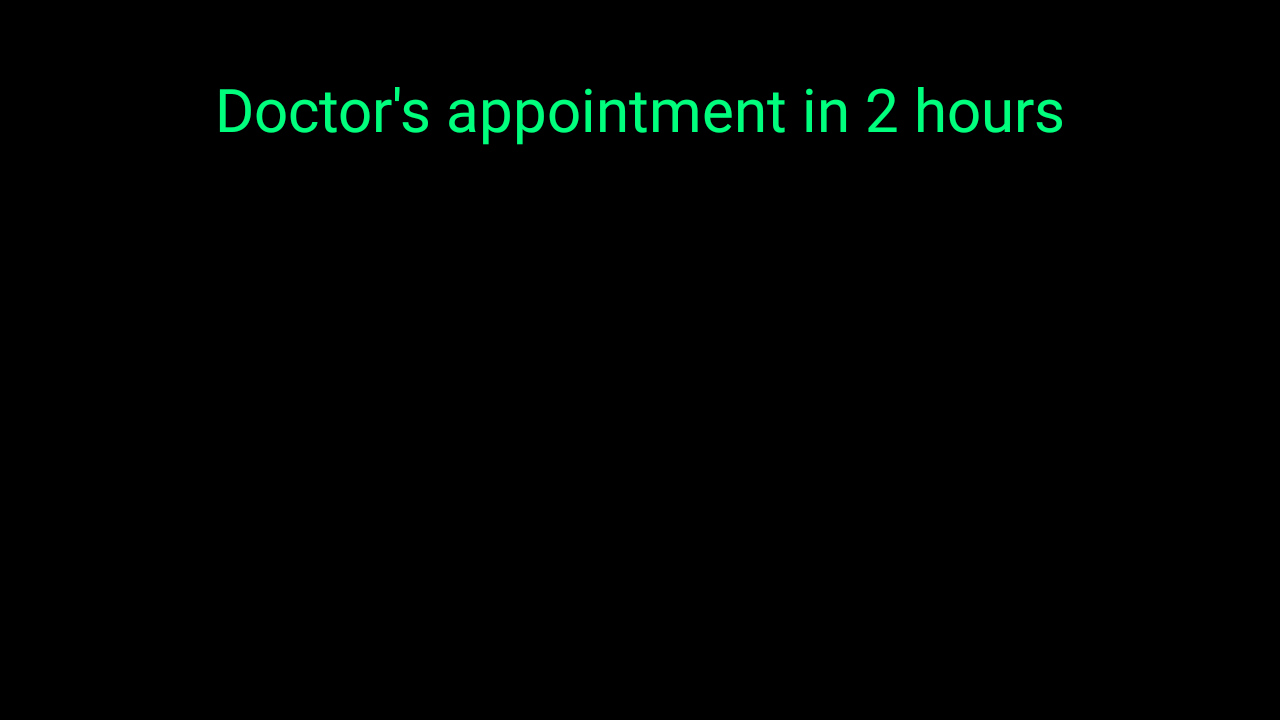
\includegraphics[width=0.95\linewidth]{\Pic{study1/layout_text_notification.png}}
  \caption{\Textnotif{} on OHMD}\label{fig:IconNotif:study1:notification_layout_text}	  
\end{subfigure}%
\begin{subfigure}{.50\linewidth}
  \centering
  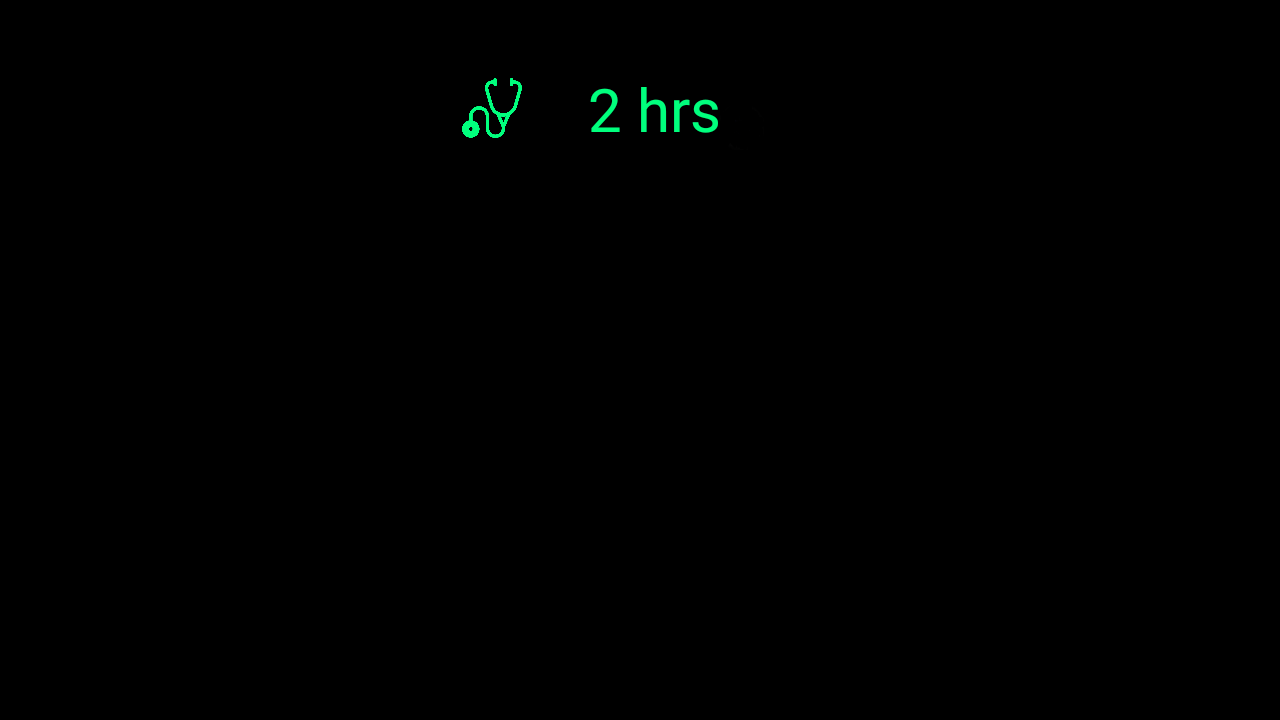
\includegraphics[width=0.95\linewidth]{\Pic{study1/layout_icon_notification.png}}
  \caption{\Iconnotif{} on OHMD}\label{fig:IconNotif:study1:notification_layout_icon}	  
\end{subfigure}
\caption[The notification layout on OHMD]{The notification layout on OHMD. The notifications are displayed at the top-center position. (a) A \textnotif{} on OHMD. (b) An \iconnotif{} on OHMD. Note: Black color in OHMD represents the transparent background. Icon source: \flatIcons{}.}
\label{fig:IconNotif:study1:notification_layout}
\end{figure}







\section{Research approach and overview}
\label{sec:IconNotif:overview:goals}

This research seeks to achieve two goals: one practical and one theoretical.
The former goal investigates whether the new \iconnotif{s} design can outperform text-based notifications in OHMD multitasking scenarios, while the latter aims to elucidate the conflicting reports in notification literature regarding the efficacy of pictograms. Hence, this research commences with a study addressing the first goal and iteratively probes the problem space based on empirical findings. 



\subsection{\Studyone{}: Compare \textnotif{s} vs \iconnotif{s} for \i{researcher-selected} icons}

In the first study (\autoref{sec:IconNotif:study1}), we compared the \iconnotif{s} design with regular \textnotif{} in a controlled multitasking scenario.
The results indicated that \iconnotif{s} outperform regular \textnotif{s} in terms of task performance and distraction reduction. While this finding suggests that the proposed \iconnotif{s} may be advantageous over \textnotif{s}, it does not address the second goal. A thorough examination of the study design revealed a potential confounding variable: filler words (e.g., linking words between \primaryinfo{} and \secondaryinfo{}, see \autoref{fig:IconNotif:overview:notification_mapping}). Due to the differing affordances between icon-augmented and text-based notifications, filler words were retained in \textnotif{s} but not in \iconnotif{s}, leading to participants spending additional time reading regular \textnotif{s}. This confounding variable hampers conclusive interpretations regarding the superiority of pictograms over text.


\subsection{\Studytwo{}: Compare \iconnotif{s} and transformed \textnotif{s} for \i{researcher-selected} icons}

To mitigate this potential bias, we removed the filler words from \textnotif{s} and conducted a second study (\autoref{sec:IconNotif:study2}, see \autoref{fig:IconNotif:study2:notification_mapping}). Before commencing this study and to ensure the comprehensibility of the resulting \textnotif{s}, we conducted a pilot study with four participants. The results suggested that removing filler words in \textnotif{s} did not significantly affect their comprehension.

Upon analyzing the \studytwo{} results, we observed that the previously noted statistical advantages of \iconnotif{s} from \studyone{} had vanished, even though most participants still subjectively preferred \iconnotif{s}. The study results indicated that apart from subjective preferences, replacing text with icons does not confer any statistically significant advantage.

While this finding aligns with past studies that found no advantage for pictograms over text, it fails to explain why some previous studies did report advantages for pictograms. After closely examining the design of the first two studies, we identified two additional potential influencing factors: content familiarity and \encodingcomplexity{}.

Regarding content familiarity, the participants were more familiar with text stimuli due to their daily use for many years; in contrast, they had less exposure to the icons used in the experiment and were unfamiliar with the meanings of all icons. Although we attempted to bridge this gap with training and practice before the experiment, post-experimental feedback revealed that participants still lacked familiarity with some of the icons used in the experiment, which could potentially bias the results.

As for \encodingcomplexity{}, it refers to the number of words an icon represents and is another potential influential factor. For example, \inlineimg{\Pic{icons/img_car4.png}} represents `Car', a single word, while \inlineimg{\Pic{icons/img_no_left_turn.png}} stands for `No Left Turn', which comprises three words. The higher the encoding density, arguably, the more efficient the encoding process in the brain, which can affect the efficacy of notification recognition.

\subsection{\Studythree{}: Compare \iconnotif{s} with transformed \textnotif{s} for \i{user-selected} icons}

To better understand how these two factors may influence the results obtained from \studytwo{}, we conducted a third study (\autoref{sec:IconNotif:study3}, \autoref{fig:IconNotif:study3:notification_mapping}). This study aimed to improve the participants' familiarity with the selected icons and incorporated \encodingcomplexity{} as another independent variable. In this study, rather than providing a predefined set of icons as stimuli, we allowed participants to choose their own icons, thereby potentially increasing their familiarity with the stimuli.

The \studythree{} results showed that: 1) with increased familiarity, \iconnotif{s} regained their statistical advantage over \textnotif{s}, and 2) an interaction effect was found between the presentation \format{} $\times{}$ \i{\encodingcomplexity{}}. A detailed analysis revealed that the observed advantages in \iconnotif{s} are primarily attributed to the higher \complexity{} conditions but not the lower ones.

By integrating the findings of the three studies, we can deduce a plausible explanation for the inconsistent results observed in the literature. This explanation suggests that many factors influence the performance comparison of pictograms and text. Pictograms can outperform text in multitasking performance, given several conditions: 1) the pictogram's design needs to be intuitive and unambiguous, 2) users must be highly familiar with the pictogram, and 3) the \complexity{} of the pictogram must be high. If any of these conditions are not met, the advantages of pictograms may not materialize.


\subsection{\Studyfour{}: Compare \iconnotif{s} and transformed \textnotif{s} in realistic settings for \i{user-selected} icons}

Evaluating the performance of \iconnotif{s} on OHMDs in real-life settings can provide better insights into how pictograms compare with text. Therefore, we conducted a fourth study (\autoref{sec:IconNotif:study4}) in realistic stationary and mobile settings to validate the generalizability of laboratory findings. The results largely confirmed the laboratory studies' findings, where carefully designed \iconnotif{s} can reduce distraction compared to text. However, it also revealed additional factors influencing users' performance, such as the amount of external lighting.

The sections above provide an overview of the current research. The following sections will present each of the above studies in detail.


\subsection{Common setting}

All three controlled studies (\Studyone{, 2, and 3}) were based on a dual-task scenario \cite{pashler_dual_task_1994}. These studies aimed to validate whether adapting pictorial representation reduces attention costs while retaining content delivery. We selected a \i{vigilance task} (an attention-demanding, perceptual monitoring task) as the primary task, for which attentional control was measured \cite{ramachandran_vigilance_2002, redick_cognitive_2016}. Users were instructed to attend to the calendar notifications as the secondary task. Similar approaches have been used to measure the attentional cost of mobile phone notifications \cite{stothart_attentional_2015} and multitasking on OHMDs \cite{mustonen_visual_2013, klose_text_2019}.








\section{Study 1: Compare \textnotif{s} vs \iconnotif{s} for \textit{researcher-selected} icons}
\label{sec:IconNotif:study1}

In this study, we compared \textnotif{s} and \iconnotif{s} with the \nonotif{} condition, evaluating both task performance and user preference. 

\subsection{Participants}
\label{sec:IconNotif:study1:participants}

Sixteen volunteers (8 females, 8 males; mean age = 22.7 years, SD = 2.5) participated in this study. All participants had normal or corrected-to-normal visual acuity with no reported color or visual deficiencies/impairments. Participants were from the university community, had self-reported professional working fluency in English, and were avid smartphone users who received, on average 51 (min = 30, max = 100) daily notifications. However, none had prior experiences with OHMDs. 

In \b{all} studies, participants gave consent and were compensated at a rate of approximately USD 7.25/hour. \b{None} of the participants in any study participated in subsequent studies.

\subsection{Apparatus}
\label{sec:IconNotif:study1:apparatus}

The study was conducted in a quiet room under indoor lighting conditions to provide a consistent user experience and avoid environmental interference \cite{gabbard_effects_2006, debernardis_text_2014}. 

The primary task was displayed on a light grey background on a 23'' LCD monitor (refresh rate = 60 Hz, resolution = 1920 x 1080 px) at eye level (see \autoref{fig:IconNotif:study1:aparatus}), and was designed using PsychoPy \cite{peirce_psychopy2_2019}, a Python library used for experimental psychology research.

The stimuli of the primary task and notifications were presented at different depths to simulate attention switching between physical and virtual backgrounds. Thus, the participant's eyes were set to be 70 cm away from the computer monitor, which differs from the focal length of around 1m \cite{laramee_rivalry_2002} used by OHMDs. 

Notifications were presented on Epson Moverio BT-300 smart glasses \cite{epson_tech_2020} (\autoref{fig:IconNotif:studay1:smart_glasses}), a binocular OHMD with 1280x720 px (30Hz) resolution display, 23$^{\circ}$ FoV, and a projected distance of 80 inches at 5m, running on Android 5.1 OS (headset weight = 69 g).
We selected the BT-300 as it provides a subset of the functionalities/features found in more advanced OHMDs (such as HoloLens2, Nreal Light, etc.), meaning that our results can be better generalized to a wide range of OHMDs (details at \autoref{sec:IconNotif:general_discussion:generalizing_ohmds}).

We installed a custom-developed Android application on the OHMD to display custom notifications (\autoref{fig:IconNotif:study1:notification_layout}). A Python program controlled the stimuli displayed on the monitor, pushed notifications to the OHMD, logged user inputs, and synchronized timings. Implementation details are provided at \autoref{sec:IconNotif:programming_codes}.

\begin{figure}[hptb]
\centering

\begin{subfigure}{.50\linewidth}
  \centering
  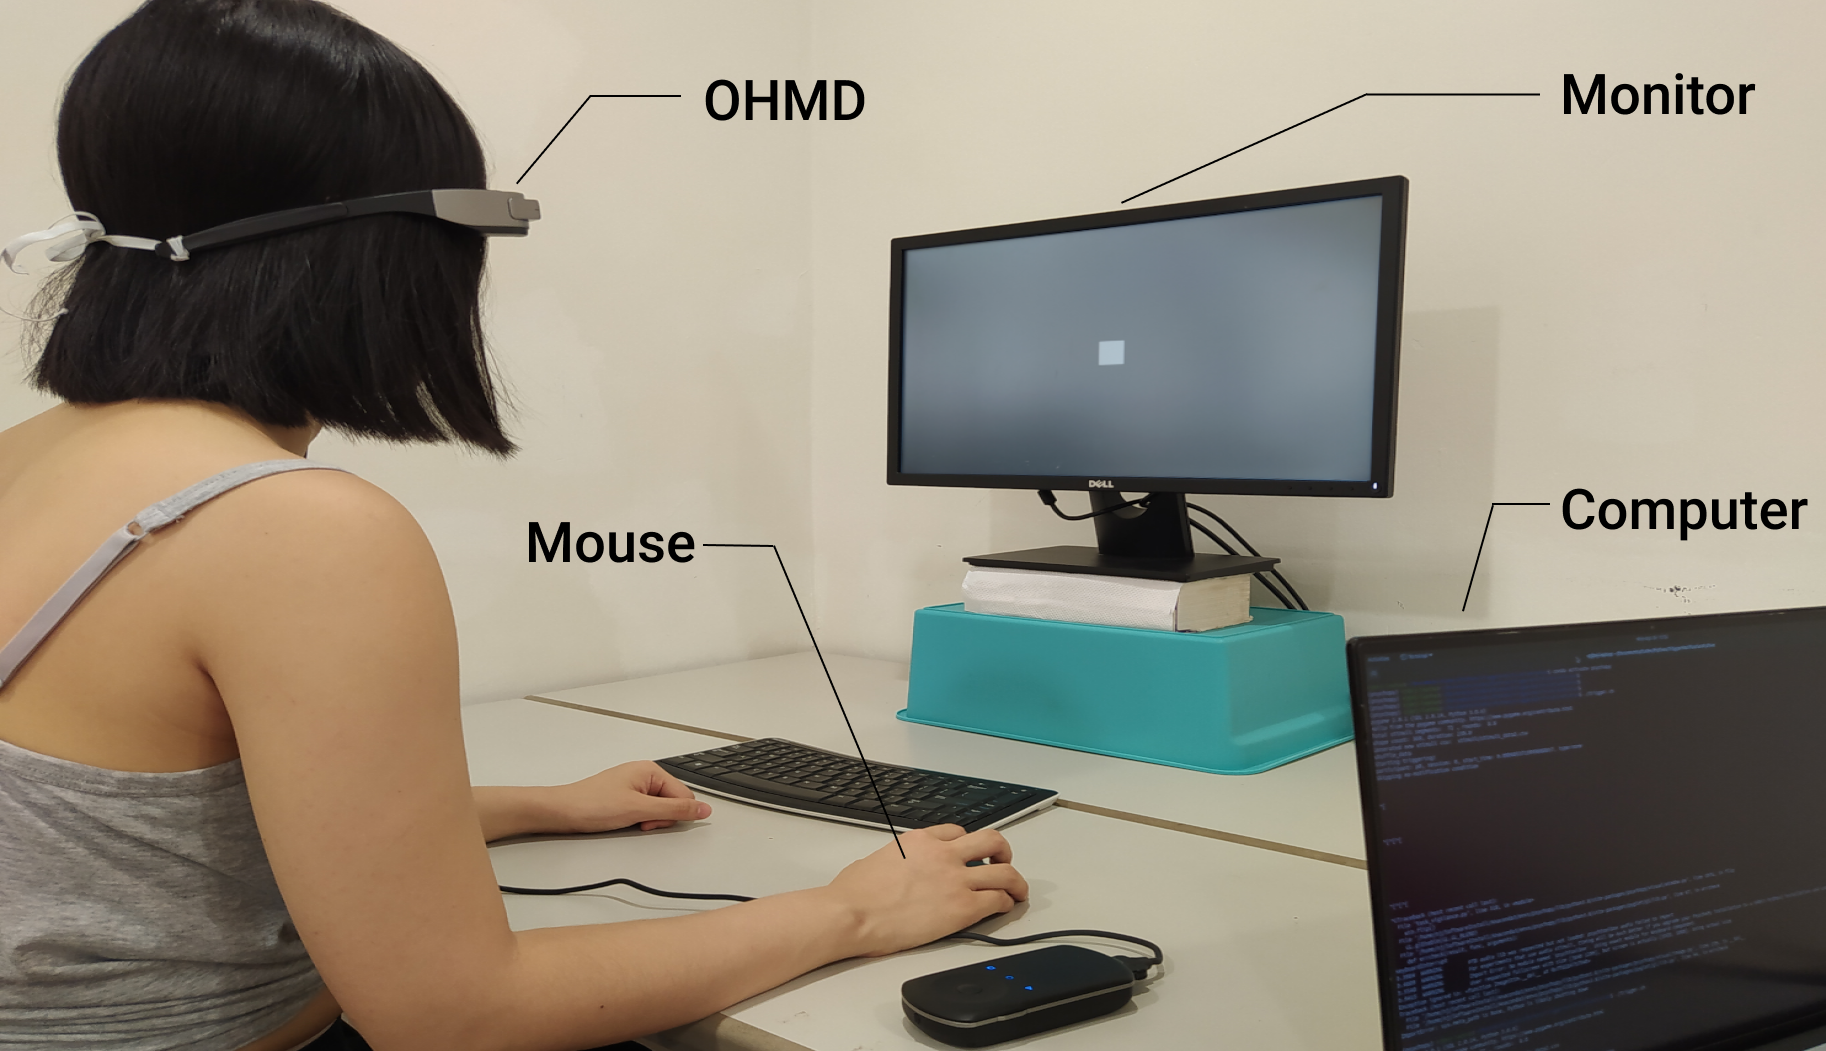
\includegraphics[width=0.95\linewidth]{\Pic{study1/aparatus.png}}
  \caption{Apparatus setup}
  \label{fig:IconNotif:study1:aparatus}	  
\end{subfigure}%
\begin{subfigure}{.50\linewidth}
  \centering
  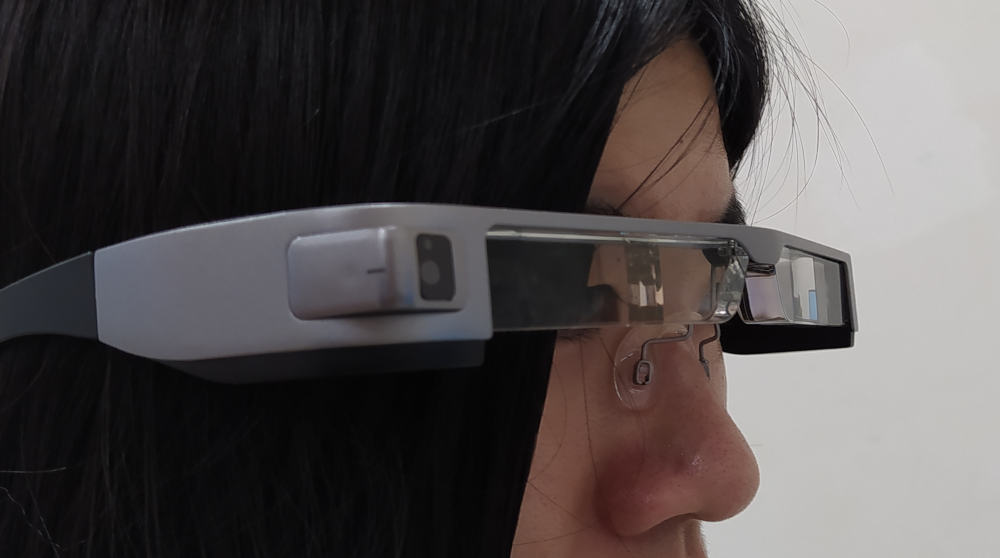
\includegraphics[width=0.96\linewidth]{\Pic{study1/smart_glasses.png}}
  \caption{Epson BT-300 smart glasses}
  \label{fig:IconNotif:studay1:smart_glasses}	  
\end{subfigure}

\caption[Apparatus in the controlled experiments]{Study apparatus used in the controlled experiments.}
\label{fig:IconNotif:study1:setup}
\end{figure}



\subsection{Tasks}
\label{sec:IconNotif:study1:task}

For the \i{primary (vigilance) task}, we adopted the shape detection task developed by Santangelo et al. \cite{santangelo_perceptual_2008} and reused by Mustonen et al. \cite{mustonen_visual_2013} to evaluate visual task performance on an OHMD.

We chose this vigilance task for two reasons. Firstly, the vigilance task is an established representative task simulating real-world usage of OHMDs in dynamic and unpredictable environments \cite{mustonen_visual_2013}. This is particularly relevant in situations where attention needs to be divided between the display (virtual content: notifications) and the environment (physical content: shape detection), such as walking in crowded areas. Moreover, this task can measure the degradation of sustained visual attention and perceptual monitoring capabilities when receiving virtual content, which impacts gaze, attention, and situational awareness \cite{mustonen_visual_2013, nenna_augmented_2021}. Secondly, a controlled experimental task ensures a fair comparison. Although real-world tasks have higher external validity, they often introduce many confounding variables that are difficult to control.
 
During the shape detection task, visual stimuli continuously morphed between small (15 x 15 $mm^{2}$) and large (30 x 30 $mm^{2}$) white squares over 625 ms in segments lasting 3750 ms. These small and large white squares are non-targets (\autoref{fig:IconNotif:study1:vigilance_task}). A target shape, either a vertical (15 x 30 $mm^{2}$) or horizontal (30 x 15 $mm^{2}$) rectangle, randomly appeared in 88.9\% of segments, with no two rectangles appearing within 1875 ms of each other. Participants were instructed to press the left mouse button upon detecting a target rectangle shape within a time limit of 1875 ms. The total duration of the task was four minutes (=236,250 ms) to ensure sufficient time for assessing participants' attention control \cite{mustonen_visual_2013}. 


\begin{figure}[hptb]
  \centering
  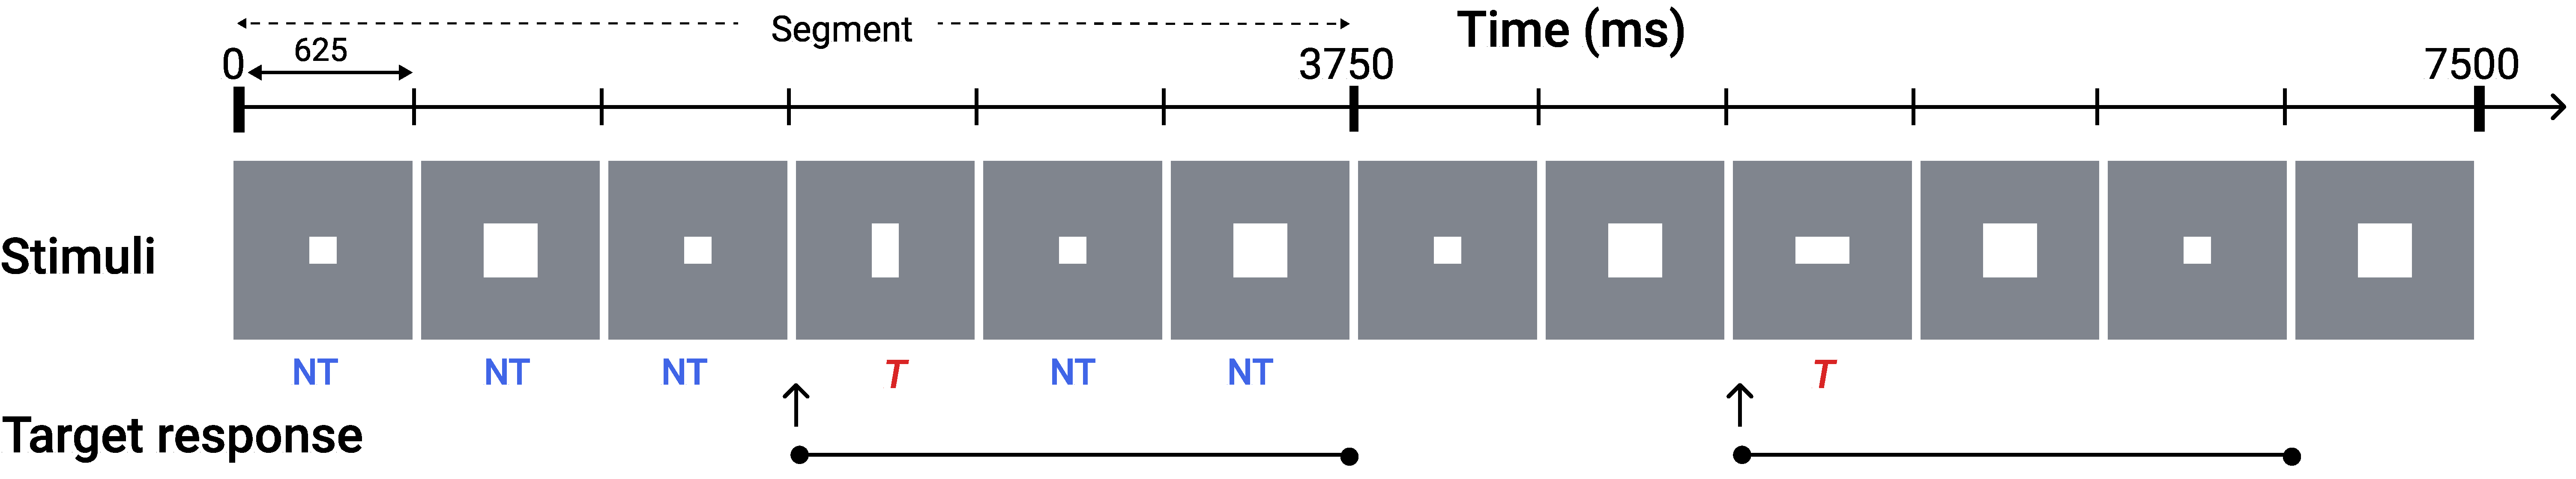
\includegraphics[width=\linewidth]{\Pic{study1/vigilance_task.pdf}}
  \caption[The stimulus in controlled experiments]{The stimulus is a square (non-targets = NT) that morphs between small and large sizes in cycles of 625 ms. The stimulus morphed into the target shape (T = vertical or horizontal rectangle) randomly, and participants were instructed to respond by pressing their mouse button within 1875 ms. This figure depicts the square shapes morphing to target shapes in $4^{th}$ morph in $1^{st}$ segment (0-3750 ms) and $3^{rd}$ morph in $2^{nd}$ segment (3750-7500 ms). Note: stimuli are not drawn to scale.}
  \label{fig:IconNotif:study1:vigilance_task}	  
\end{figure}

The \i{secondary (notification) task} was to attend to the calendar notifications on the OHMD. Six notifications were randomly displayed during the primary task, with a minimum interval of 20 seconds between each notification and a display duration of 10 seconds, similar to the study conducted by Rzayev et al. \cite{rzayev_effects_2020}. The calendar notifications designed in \autoref{sec:IconNotif:overview:icon_notif_design} were used in this task.


\subsection{Study design and procedure}
\label{sec:IconNotif:study1:design_procedure}

A repeated-measures within-subject design was used to investigate the participants' performance on primary and secondary tasks for three notification presentation formats: \textnotif{}, \iconnotif{}, and \nonotif{}, with the latter being used as the comparative baseline. The experiment consisted of three testing blocks, each with a duration of four minutes, which were counterbalanced using a Latin square.



\subsubsection*{Procedure}
\label{sec:IconNotif:study1:procedure} 

Participants were first instructed to familiarize themselves with the \textit{researcher-selected} icon-to-text mapping (\autoref{sec:IconNotif:overview:notification_design}).

Next, two verbal recognition tests were administered on OHMD to verify the participants' icon recognition accuracy for all icons. The notifications related to the icons that participants recognized wrongly in the second test were removed before the training and testing blocks to minimize the effects of unfamiliar/unintuitive icons. The resulting notifications (22-24 per participant) were used by the apparatus (\autoref{sec:IconNotif:study1:apparatus}) to show notifications randomly without repetition.

Afterward, a training session for at least two minutes each in all conditions was conducted until participants felt comfortable with the apparatus, tasks (primary and secondary), and questionnaires. Then, the participants underwent three testing blocks knowing the condition and were instructed to attend to the primary task as quickly and accurately as possible. At the end of each block, participants completed a questionnaire that recorded their perceived behaviors and recalled notifications. A minimum break of two minutes with eye exercises was given between blocks to minimize fatigue.

Upon completing all blocks, participants completed a questionnaire with their overall rankings for each format. They attended an 8-12 minutes semi-structured post-interview in which they were asked about the reasons for each ranking, the process, and the multitasking experience with different formats. Each experiment comprised one session lasting 40-55 minutes. 




\subsection{Measures}
\label{sec:IconNotif:study1:measures}

\subsubsection*{Primary (vigilance) task}

Both accuracy and speed are measured for the primary task.
To measure the accuracy, \textit{hit rate} (\hitrate{} = $\frac{\#hit}{\#hit + \#miss} \in [0,1]$, $hit$ = correct identification of target shape) and \textit{false alarm rate} (\falsealarmrate{}\footnote{Since $target\:\%$ = 88.9\% > $noise\:\%$ = 10.1\%, the precision of \falsealarmrate{} is lower than that of  \hitrate{}} = $\frac{\#false\:alarm}{\#false\:alarm + \#correct\:rejection} \in [0,1]$, $false \: alarm$ = misidentifying a noise signal as a target signal) were used; while to measure speed, \textit{reaction time} (\reactionTime{}= response time - target stimuli start time, in $seconds$) was used. A failure to respond within the time limit was considered a miss, and reaction times were calculated only for the hits.

\subsubsection*{Secondary (notification) task}

As mentioned in \autoref{sec:Relatedwork:notification_evaluation}, we used the IRC framework to evaluate the proposed \iconnotif{s} as shown in \autoref{tab:IconNotif:study1:IRC_measure}.

\begin{table}[hptb]
\centering
\caption[Measures based on IRC framework]{Measures based on IRC framework \cite{chewar_unpacking_2004, mccrickard_model_2003, mccrickard_attuning_2003}. Here [O] represents objective measures while [S] represents subjective measures.}
\label{tab:IconNotif:study1:IRC_measure}
\small
\begin{tabular}{@{}ll@{}}
\toprule
Parameter & Measures \\ \midrule
\Interruption{} &  [S] Perceived cost of interruption (task load) \\
\Reaction{} &  [S] Immediate response (noticeability) \\
\Comprehension{} &  [O] Base comprehension (recall accuracy and understandability) \\
\Satisfaction{}  & [S] Preference \\ 
\bottomrule
\end{tabular}
\end{table}



\factor{\Interruption{}}
\textit{Perceived task load} using raw NASA-TLX (\perceivedTaskLoad{}, 0-100 scale) \cite{nasa_tlx_2006}, \perceivedInterruption{} (`How much interruption did the notification cause to the task when you attempt to carry out both simultaneously?') using a 0-100 visual analogue scale, and distraction ranking were used to measure the perceived cost of interruption. 


\factor{\Comprehension{}}
Immediate recall accuracy (\immediateRecall{}) and understandability ranking were used to measure the comprehension of each \format{}. \immediateRecall{} was calculated for the notifications displayed while participants were engaged with the primary task, using a questionnaire after each block. 
\immediateRecall{} was used in this study in order to simulate the scenario where certain calendar notifications need to be remembered to take due action in the future \cite{tungare_exploratory_2008, kelley_how_1982}.
For each correct \primaryinfo{}, 0.5 points were assigned, and another 0.5 points were assigned to correct \secondaryinfo{} when \primaryinfo{} was correct.
Consider a hypothetical case where a participant sees two notifications, `<meeting, 4 pm>' and `<birthday, tomorrow>'. If the participant recalled only one notification, `<meeting, tomorrow>' (e.g., the participant wrote `meeting is on tomorrow' in the questionnaire), they would get only 0.5 points since `tomorrow' (\secondaryinfo{}) is not the correct secondary info for `meeting'(\primaryinfo{}). Since six notifications were displayed during testing blocks, participants could score a maximum of 6 points for \immediateRecall{} in each \textnotif{} or \iconnotif{} \format{}.

\factor{\Reaction{}}
Noticeability ranking was measured to understand how \format{} affects the rapid detection of notifications.

\factor{\Satisfaction{}}
Overall user preference ranking was used to measure the desirability of each \format{}.




\subsection{Results}
\label{sec:IconNotif:study1:results}

Every participant completed three blocks, receiving 12 notifications and 192 targets. They scored a minimum of 3 (out of 6) for recall accuracy and had more than 72\% hit rate at the end of each notification block. Data from one participant was discarded as an outlier due to a hit rate deviation that exceeded three times the standard deviation from the mean. \autoref{tab:IconNotif:study1:mean_results} presents the mean performance of measures for the participants.

\begin{table*}[hptb]
\caption[Average performance in \studyone{}]{\Studyone{} performance in dual-task scenario (N = 15). Colored bars show the relative value of each measure for different notification formats. \significantI{} \significantII{} \significantIII{} represent significant post-hoc tests (\pbonf{<0.05}). Here, \i{Text} = \textnotif{}, \i{Icon} = \iconnotif{}, \i{No} = \nonotif{}, \hitrate{} = \textit{hit rate}, \falsealarmrate{} = \textit{false alarm rate}, \reactionTime{} = \textit{reaction time}, and \perceivedTaskLoad{} = \textit{Raw NASA-TLX score}.}
\label{tab:IconNotif:study1:mean_results}
\centering
\small
\begin{tabular}{@{}l|ll|ll|ll@{}}
\toprule
\multicolumn{1}{r}{Measure} &
  \multicolumn{2}{c}{\hitrate{}} &
  \multicolumn{2}{c}{\falsealarmrate{}} &
  \multicolumn{2}{c}{\reactionTime{}} 
  \\ \cmidrule(l){1-7} 
\multicolumn{1}{l}{Format} &
  \multicolumn{1}{|l}{M} &
  \multicolumn{1}{l}{SD} &
  \multicolumn{1}{l}{M} &
  \multicolumn{1}{l}{SD} &
  \multicolumn{1}{l}{M} &
  \multicolumn{1}{l}{SD} \\ \midrule
  
\i{No} & 
\databarrel{0.98}{0.8}{0.960}\significantII{}\significantIII{} & 0.042 & 
\databar{0.5}{0.052} & 0.108 & 
\databarrel{0.49}{0.44}{0.464}\significantI{} & 0.044
\\

\i{Icon} & 
\databarrel{0.98}{0.8}{0.938}\significantI{}\significantIII{} & 0.055 & 
\databar{0.5}{0.073} & 0.147 & 
\databarrel{0.49}{0.44}{0.479} & 0.039 
\\

\i{Text} & 
\databarrel{0.98}{0.8}{0.923}\significantI{}\significantII{} & 0.057 &
\databar{0.5}{0.086} & 0.134 & \databarrel{0.49}{0.44}{0.486}\significantI{} & 0.050 
\\

\bottomrule
\end{tabular}

\small
\begin{tabular}{@{}l|ll|ll|ll@{}}
\toprule
\multicolumn{1}{r}{Measure} &
\multicolumn{2}{c}{\immediateRecall{}}  &
  \multicolumn{2}{c}{\perceivedTaskLoad{}} &
  \multicolumn{2}{c}{\perceivedInterruption{}} 
  \\ \cmidrule(l){1-7} 
\multicolumn{1}{l}{Format} &
  \multicolumn{1}{l}{M} &
  \multicolumn{1}{l}{SD} &
  \multicolumn{1}{l}{M} &
  \multicolumn{1}{l}{SD} &
  \multicolumn{1}{l}{M} &
  \multicolumn{1}{l}{SD} \\ \midrule
  
\i{No} & 
- & - &
\databar{60}{29.17}\significantI{}\significantII{} & 17.35 &  
- & - 
\\

\i{Icon} & 
\databar{5}{4.83} & 0.88&
\databar{60}{48.33}\significantII{} & 16.75 & 
\databar{70}{52.00}\significantI{} & 21.36 
\\

\i{Text} & 
\databar{5}{4.80} & 0.75 &
\databar{60}{55.17}\significantI{} & 18.37 & 
\databar{70}{63.67}\significantI{} & 20.91 
\\

\bottomrule
\end{tabular}

\end{table*}



\subsubsection*{Analysis}
\label{sec:IconNotif:study1:analysis}

Quantitative data were analyzed using a one-way repeated measures ANOVA when baseline data were available; if ANOVA assumptions were violated, the Friedman test was applied. A paired-sample t-test or Wilcoxon signed-rank test with Bonferroni correction was used for cases without baseline data. Data normality was tested using the Shapiro-Wilk test, and sphericity was assessed using the Mauchly test. As suggested by Huberty and Morris \cite{huberty1992multivariate}, each dependent variable was subjected to statistical tests individually due to their conceptually distinct aspects. Parametric tests were applied when non-parametric distributions could assume a wide range of values and met parametric assumptions. 

Interview recordings were transcribed and thematically analyzed as outlined by Braun and Clarke \cite{braun_using_2006}. Qualitative findings were categorized into themes to either support or oppose quantitative findings.


\subsubsection*{Primary (vigilance) task performance}
\label{sec:IconNotif:study1:primary_task_performance}

As anticipated, both notification \format{s} significantly reduced the primary task's accuracy (i.e., low hit rate, high false alarm rate) and speed (i.e., low reaction time), demonstrating that notifications impair the performance of the primary task.

However, \iconnotif{} exhibited a higher hit rate, a lower false alarm rate, and a shorter reaction time than \textnotif{}, suggesting that \iconformat{} is more capable of maintaining primary task performance than \textformat{}. 

\begin{itemize}
    \item \i{Hit rate}: A Friedman test revealed a significant effect of notification format (\friedman{2}{6.778}{=0.035}{0.709}, strong agreement\footnote{0.3 $\leq{}$ W $<$ 0.6 indicates moderate agreement and 0.6 $\leq{}$ W indicates strong agreement \cite{gibbons_nonparametric_2020, tomczak_need_2014}}). Pair-wise Wilcoxon signed-rank tests with Bonferroni correction indicated that the hit rate for \nonotif{} (\meansd{0.960}{0.042}) was significantly higher (\pbonf{<0.05}) than that for \iconnotif{} (\meansd{0.938}{0.055}) and \textnotif{} (\meansd{0.923}{0.057}), and that \iconnotif{} was significantly higher (\wilcoxonef{69.5}{=0.050}{0.527}, large effect\footnote{0.3 $\leq{}$ $r$ $<$ 0.5 indicates moderate effect and 0.5 $\leq{}$ $r$ indicates large effect \cite{tomczak_need_2014, goss_sampson_statistical_2019}}) than \textnotif{}.
    % This indicates that notifications (\textnotif{} and \iconnotif{}) reduced the primary task accuracy by 2.3\%-3.9\% than when there were no notifications. In addition, we found that primary task accuracy was approximately 1.6\% lower with \textnotif{} than \iconnotif{}.

    \item \i{False alarm rate}: There was no significant difference between the notification \format{s}.


    \item \i{Reaction time}: A significant effect was observed due to the \format{} of the notification (\anovawefp{2}{28}{4.401}{=0.022}{0.239}, large effect\footnote{0.01 $\leq{}$ $\eta^{2}_{p}$ $<$ 0.06 indicates small effect, 0.06 $\leq{}$ $\eta^{2}_{p}$ $<$ 0.14 indicates medium effect, and 0.14 $\leq{}$ $\eta^{2}_{p}$ indicates large effect \cite{tomczak_need_2014, goss_sampson_statistical_2019}}). A post-hoc analysis revealed that \textnotif{} (\meansd{0.486}{0.050}) differed significantly (\pbonf{ <0.05}) from \nonotif{} (\meansd{0.464}{0.044}), but not significantly from \iconnotif{} (\meansd{0.479}{0.039}).
\end{itemize}


\subsubsection*{\Interruption{}}
\label{sec:IconNotif:study1:interruption_parameter}

Both \format{s} significantly increased cognitive load compared to \nonotif{}, but \iconnotif{} resulted in a lower cognitive load than \textnotif{}.

\begin{itemize}
    \item \i{Unweighted NASA-TLX}: A repeated-measures ANOVA demonstrated a significant effect (\anovawefp{2}{28}{45.076}{<0.001}{0.763}, large effect). A post-hoc analysis with Bonferroni corrections revealed significant differences (\pbonf{<0.05}) between \nonotif{} (\meansd{29.17}{17.34}) and both \textnotif{} (\meansd{55.17}{18.37}) and \iconnotif{} (\meansd{48.33}{16.75}). However, \textnotif{} was not significantly different (\pbonf{=0.069}) from \iconnotif{}. Individual index results are given in \autoref{fig:IconNotif:study1:nasa_tlx}. The same analysis showed significant main effects of \format{} on the overall score and all individual indices (\pval{<0.001}), except for \i{Physical Demand}. Post-hoc analysis with Bonferroni correction demonstrated that \nonotif{} had significantly lower (\pbonf{<0.001}) task load results than both \textnotif{} and \iconnotif{} for all measures except \i{Physical Demand}. \iconnotif{} was marginally significantly lower (\pbonf{<0.10}) than \textnotif{} for the overall score and \i{Frustration}.
    % To sum up, notifications led to significantly higher cognitive load than \nonotif{}, though \iconnotif{} led to a 6.8 decrease in cognitive load than \textnotif{}.
    
    \item \i{Perceived interruption}: A paired-sample t-test indicated that \textnotif{} (\meansd{63.7}{20.9}) was significantly more interruptive (\ttestef{14}{2.93}{=0.006}{0.756}, medium effect\footnote{0.2 $\leq{}$ $d$ $<$ 0.5 indicates small effect, 0.5 $\leq{}$ $d$ $<$ 0.8 indicates medium effect, and 0.8 $\leq{}$ $d$ indicates large effect \cite{tomczak_need_2014, goss_sampson_statistical_2019}}) than \iconnotif{} (\meansd{52.0}{21.4}).
    % Thus, transformation is ideal as \iconnotif{} scored 11.7 lower in perceived interruption than \textnotif{}.
    
    \item \i{Distraction ranking}: Eleven out of fifteen participants perceived \textnotif{} as the most distracting to their primary task as they often had to read the text in multiple glances, and it took longer to absorb the information compared to \iconnotif{}. Three participants found \iconnotif{s} more distracting due to their unfamiliarity. The remaining participant found both formats equally distracting.
\end{itemize}


\begin{figure}[hptb]
  \centering
  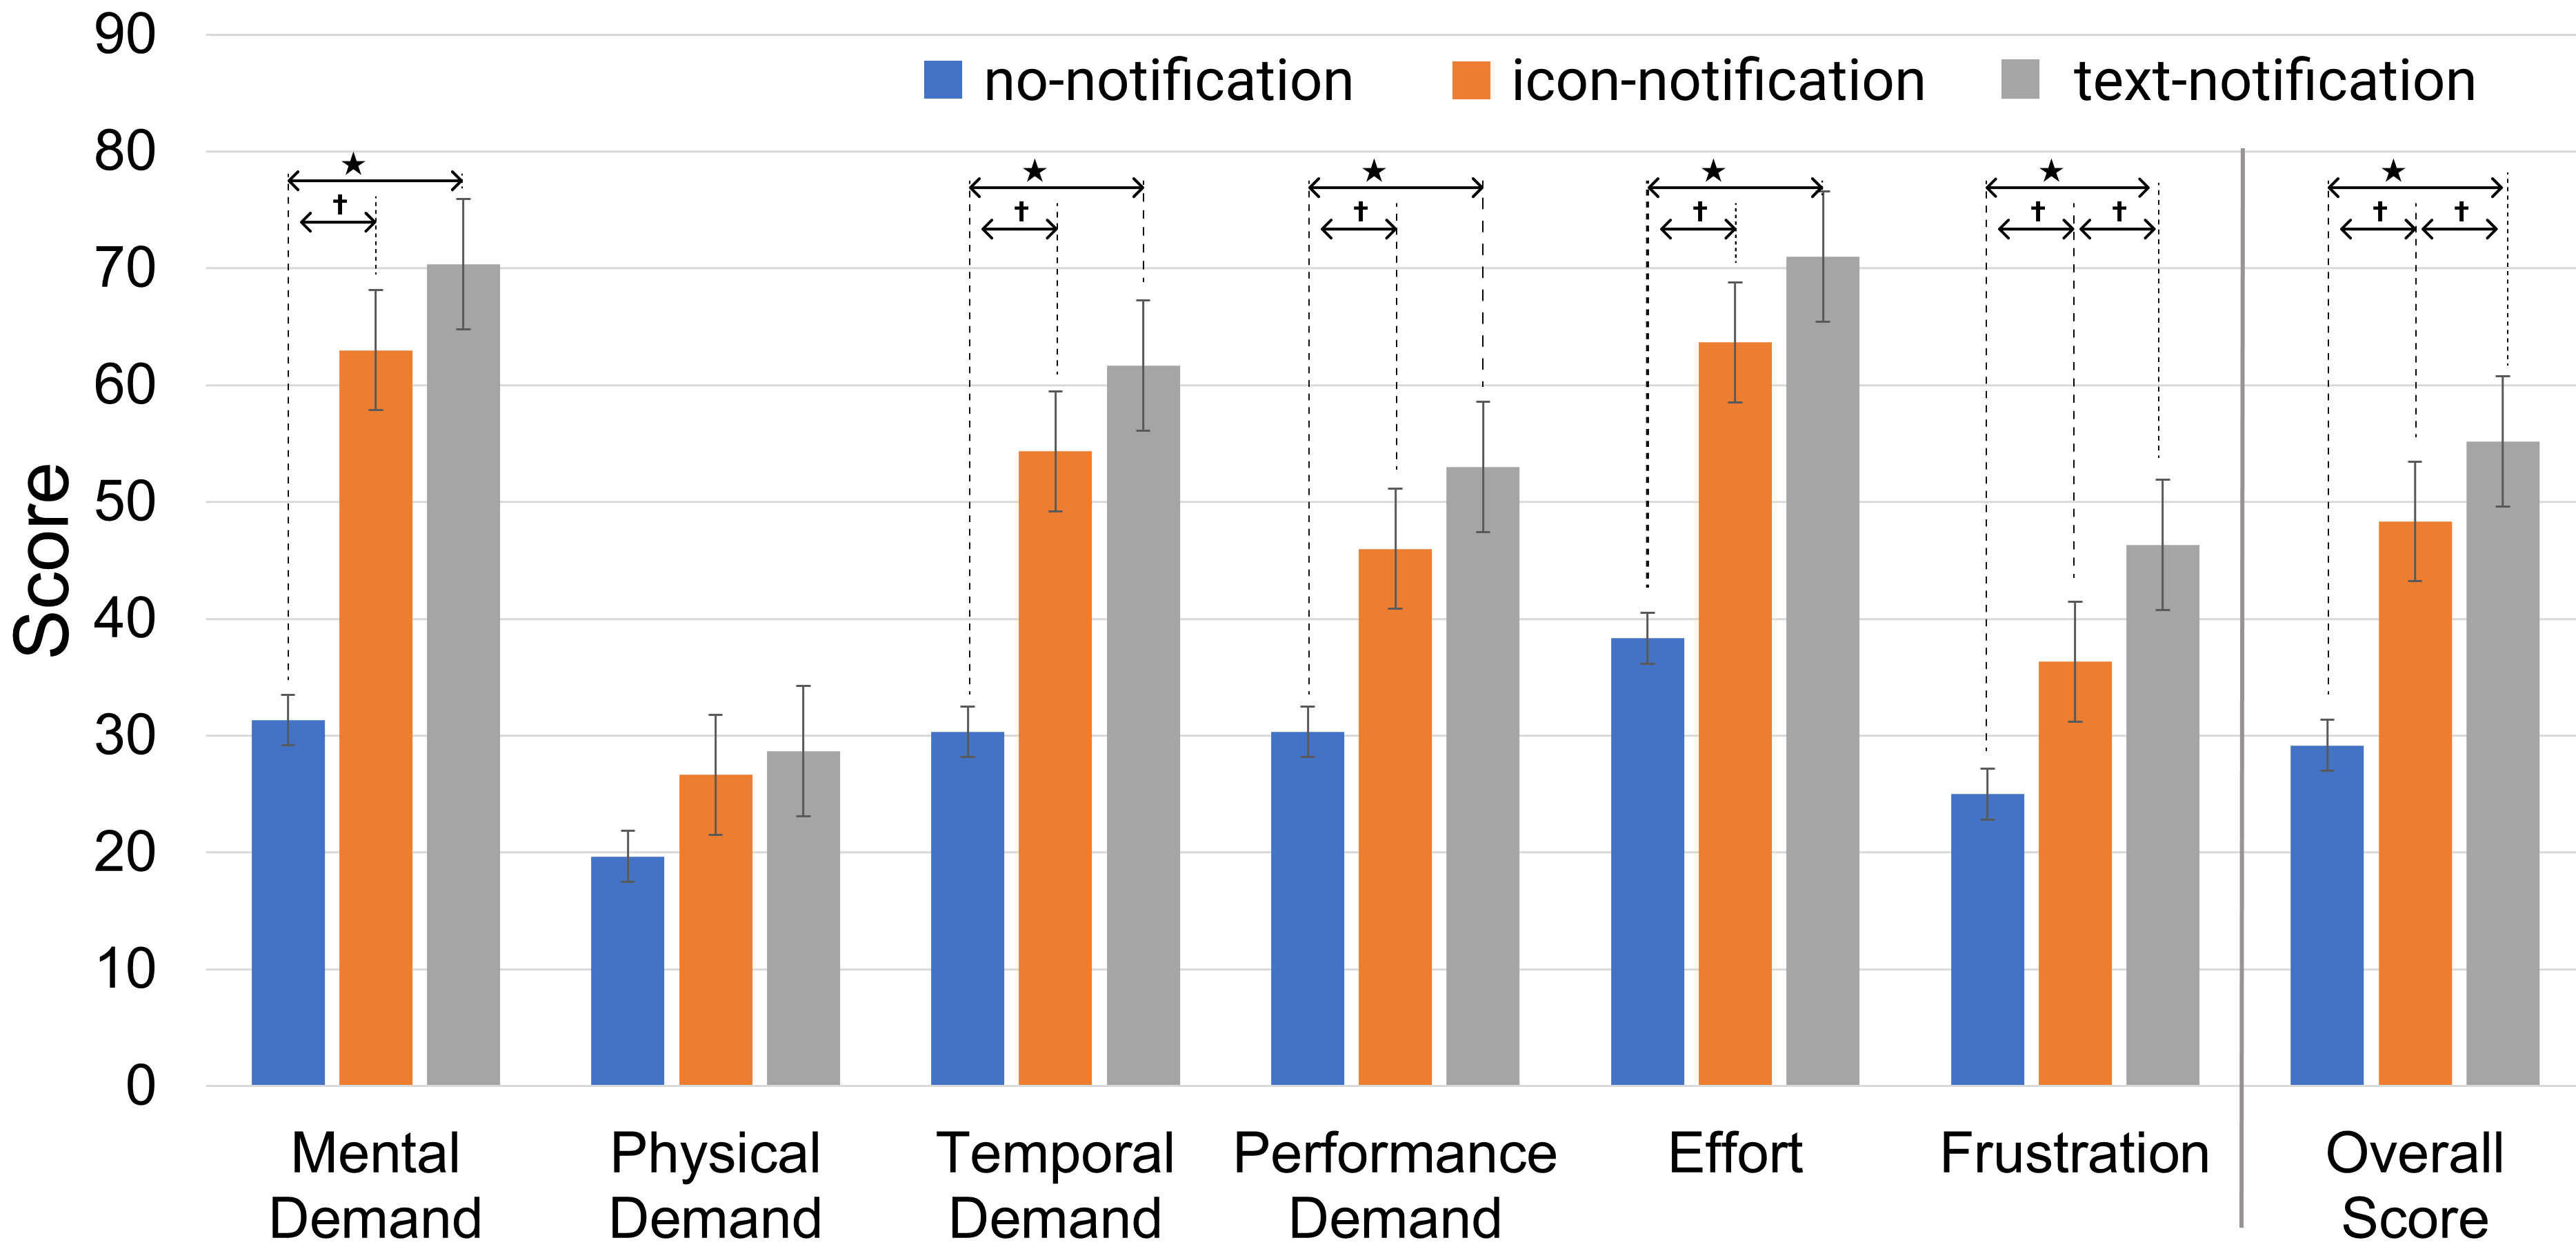
\includegraphics[width=0.9\linewidth]{\Pic{study1/study1_nasa_tlx.png}}
  \caption[NASA-TLX scores in \studyone{}]{NASA-TLX scores for \nonotif{}, \iconnotif{}, and \textnotif{} in \Studyone{} (N=15). On all indices, including overall score, the sorted order of task load from lower to higher was; \nonotif{} < \iconnotif{} < \textnotif{}. \significantI{} and \significantII{} represent significant (\pbonf{<0.05}) post-hoc tests. Error bars represent standard errors. }
  \label{fig:IconNotif:study1:nasa_tlx}	  
\end{figure}


\subsubsection*{\Comprehension{}}
\label{sec:IconNotif:study1:comprehension_parameter}
\begin{itemize}
    \item \i{Immediate recall accuracy}: A Wilcoxon signed-rank test indicated no significant difference between \iconnotif{} (\meansd{4.83}{0.88}) and \textnotif{} (\meansd{4.80}{0.75}) in terms of \immediateRecall{}. This suggests that the secondary (notification) task performance during multitasking was not influenced by the \format{}.
    
    \item \i{Understandability ranking}: An equal number of participants (six for each, or 40\%) felt that either \textnotif{s} or \iconnotif{s} were more understandable: those preferring \textnotif{s} did not need to interpret icons, while those preferring \iconnotif{s} found them shorter and easier to process mentally. The remaining three participants found both \format{s} equally understandable.
\end{itemize}


\subsubsection*{\Reaction{}}
\label{sec:IconNotif:study1:reaction_parameter}

There was no consensus among participants regarding the noticeability of the two formats.

\begin{itemize}
    \item \i{Noticeability ranking}: Seven (47\%) participants found both \format{s} equally noticeable. Five participants found \iconnotif{} more noticeable due to its pictorial distinctiveness. The remaining three participants found \textnotif{} more noticeable because of its longer length.
\end{itemize}



\subsubsection*{\Satisfaction{}}
\label{sec:IconNotif:study1:satisfaction_parameter}

All but one participant (93\%) preferred to receive \iconnotif{s}. They cited the icons' intuitive nature, brevity, less disruptive presence, and easier long-term recognition/interpretation as reasons for their preference (e.g., \quote{in the long term, I will be familiar with icons more...So subconsciously, I immediately know what it means...For text, I always have to read, even if both [\textnotif{s} and \iconnotif{s}] were the same}). 


\subsection{Discussion}
\label{sec:IconNotif:study1:discussion}

The results indicate that \iconnotif{s} significantly improved primary task performance compared to \textnotif{s}. From this, we can infer that the transformation may facilitate multitasking, as it led to enhanced performance on the primary task while preserving performance on the secondary task (i.e., recall accuracy). Similarly, \iconnotif{s} significantly reduced \Interruption{} while maintaining \Reaction{} and \Comprehension{} levels; they were also generally preferred over \textnotif{s}. These findings support the practical objectives of this study (\autoref{sec:IconNotif:overview:goals}), suggesting that \iconnotif{s} offer advantages over \textnotif{s} during multitasking.

However, participant feedback suggested that additional factors might affect the effectiveness of \iconnotif{s}. For instance, the presence of filler words in \textnotif{s} could have led participants to spend additional time reading these notifications compared to \iconnotif{s}, which used abbreviations. This feedback prompted questions regarding the impact of filler words in \textnotif{s} on multitasking effectiveness. As a result, we conducted additional studies to investigate the influence of filler words.

















\section{Study 2: Compare \iconnotif{s} and transformed \textnotif{s} for \textit{researcher-selected} icons}
\label{sec:IconNotif:study2}

To control for the impact of filler words and abbreviations, a second study was conducted comparing \iconnotif{s} with \textbf{transformed} \textnotif{s}--- from which filler words had been removed (e.g., \i{meeting at 4 pm  -> meeting  4 pm})--- using \textit{researcher-selected} icons. The same apparatus (\autoref{sec:IconNotif:study1:apparatus}) and task (\autoref{sec:IconNotif:study1:task}) utilized in the previous study were employed here.

\subsection{Participants}
\label{sec:IconNotif:study2:participants}

Twelve volunteers (7 females, 5 males, mean age = 23.4 years, SD = 2.7) participated in this study. Their backgrounds were similar to those of participants from \studyone{} (\autoref{sec:IconNotif:study1:participants}), with the exception of one participant who had previously used an OHMD for one hour.

\subsection{Revised notification design}
\label{sec:IconNotif:study2:notification_design}

The same \i{notification design} procedure as in \studyone{} (\autoref{sec:IconNotif:overview:notification_design}) was followed. Researchers selected icons to represent \primaryinfo{} and used text/numbers for \secondaryinfo{}. To unify the information content of the \iconnotif{} and \textnotif{}, the \iconnotif{} was converted back to its text format without incorporating filler words (\autoref{fig:IconNotif:study2:notification_mapping}). The three raters involved in \studyone{} evaluated both the \iconnotif{} and their \textbf{transformed} \textnotif{} counterparts to ensure information equivalence and intuitiveness. If the content of the two formats differed, the raters adjusted the \textnotif{} until a full consensus was reached. Similarly, any \iconnotif{} deemed unintuitive was revised.


\begin{figure*}[hptb]
  \centering
    \scalebox{0.9}{
    \begin{tabular}{@{}llll@{}}
    \toprule
    regular \textnotif{}   &  \multicolumn{2}{l}{\iconnotif{}} & transformed \textnotif{} \\ \midrule
    Meeting at 4 pm  &    
\includegraphics[width=6mm]{\Pic{icons/img_meeting4.png}}       & \hspace{1mm} 4 pm      & Meeting \hspace{3.5mm} 4 pm    \\
    Doctor's appointment in 2 hours & 
\includegraphics[width=6mm]{\Pic{icons/img_doctor4.png}}       & \hspace{1mm} 2 hrs    & Doctor's appointment \hspace{3.5mm} 2 hrs     \\
    \bottomrule
    \end{tabular}
    }
  \caption[\iconnotif{s} to transformed \textnotif{s} mapping]{Mapping from \iconnotif{s} to transformed \textnotif{s}. Icon sources: \flatIcons{} and \materialIcons{}.}
  \label{fig:IconNotif:study2:notification_mapping}	  
\end{figure*}


\subsection{Procedure}
\label{sec:IconNotif:study2:design_procedure}

The procedure closely mirrored \studyone{} (\autoref{sec:IconNotif:study1:design_procedure}), with the exception that the \nonotif{} condition was eliminated from the testing conditions. The \format{} was fully counterbalanced using a Latin square.

\subsection{Results}
\label{sec:IconNotif:study2:results}

Participants achieved a minimum recall accuracy score of 2 (out of 6) and a hit rate exceeding 68\% at the end of each notification block. \autoref{tab:IconNotif:study2:mean_results} presents the mean performance of the participants across measures.

Surprisingly, no significant main or interaction effects were observed for any quantitative measures. 


\begin{table*}[hptb]
\caption[Average performance in \studytwo{}]{\Studytwo{} performance in dual-task scenario (N = 12). Colored bars show the relative value of each measure for different notification formats. Here, \i{Icon} = \iconnotif{} and \i{Text} = \b{transformed} \textnotif{}.}
\label{tab:IconNotif:study2:mean_results}
\centering
\small
\begin{tabular}{@{}l|ll|ll|ll@{}}
\toprule
\multicolumn{1}{r}{Measure} &
  \multicolumn{2}{c}{\hitrate{}} &
  \multicolumn{2}{c}{\falsealarmrate{}} &
  \multicolumn{2}{c}{\reactionTime{}} 
  \\ \cmidrule(l){2-7} 
\multicolumn{1}{l}{Format} &
  \multicolumn{1}{l}{M} &
  \multicolumn{1}{l}{SD} &
  \multicolumn{1}{l}{M} &
  \multicolumn{1}{l}{SD} &
  \multicolumn{1}{l}{M} &
  \multicolumn{1}{l}{SD} 
  \\ \midrule
 
\i{Icon} & 
\databarrel{0.98}{0.8}{0.938} & 0.080 & 
\databar{0.5}{0.041} & 0.061 & 
\databarrel{0.49}{0.44}{0.481} & 0.049 
\\

\i{Text} & 
\databarrel{0.98}{0.8}{0.949} & 0.045 & 
\databar{0.5}{0.073} & 0.095 & 
\databarrel{0.49}{0.44}{0.481} & 0.043 
\\

\bottomrule
\end{tabular}


\small
\begin{tabular}{@{}l|ll|ll|ll@{}}
\toprule
\multicolumn{1}{r}{Measure} &
  \multicolumn{2}{c}{\immediateRecall{}}  &
  \multicolumn{2}{c}{\perceivedTaskLoad{}} &
  \multicolumn{2}{c}{\perceivedInterruption{}} \\ \cmidrule(l){2-7} 
\multicolumn{1}{l}{Format} &
  \multicolumn{1}{l}{M} &
  \multicolumn{1}{l}{SD} &
  \multicolumn{1}{l}{M} &
  \multicolumn{1}{l}{SD} &
  \multicolumn{1}{l}{M} &
  \multicolumn{1}{l}{SD} \\ \midrule
 
\i{Icon} & 
\databar{5}{4.17} & 1.04 & 
\databar{60}{44.10} & 14.72 & 
\databar{60}{47.92} & 20.22 
\\

\i{Text} & 
\databar{5}{4.13} & 1.31 & 
\databar{60}{45.66} & 13.55 & 
\databar{60}{50.54} & 21.00 
\\

\bottomrule
\end{tabular}

\end{table*}


\subsubsection*{Primary (vigilance) task performance}
\label{sec:IconNotif:study2:primary_task_performance}

In contrast to \studyone{}, the \iconformat{} and \textformat{} displayed no significant differences (e.g., \i{hit rate} (pictogram: \meansd{0.938}{0.080}; text: \meansd{0.949}{0.040}, \pval{=0.50}), \i{reaction time} (pictogram: \meansd{0.481}{0.049}; text: \meansd{0.481}{0.043}, \pval{=0.62})). These results suggest that when filler words are removed, the \iconformat{} advantage dissipates, as there is no significant difference in primary task measures.

\subsubsection*{\Interruption{}}
\label{sec:IconNotif:study2:interruption_parameter}

There was no significant difference in the perceived cost of interruption (e.g., \i{unweighted NASA-TLX} (pictogram: \meansd{44.10}{14.72}; text: \meansd{45.66}{13.55}, \pval{=0.55}), \i{perceived interruption} (pictogram: \meansd{47.92}{20.22}; text: \meansd{50.54}{21.00}, \pval{=0.50})). 

\begin{itemize}
    \item \i{Distraction ranking}: Contrary to the quantitative measures, qualitative feedback showed that more participants (7/12) found the \textformat{} more distracting than the \iconformat{}, citing reasons similar to those collected in \studyone{} (\autoref{sec:IconNotif:study1:interruption_parameter}). However, the difference was less pronounced than in \studyone{}. The rest of the participants thought the opposite. 
\end{itemize}

\subsubsection*{\Comprehension{}}
\label{sec:IconNotif:study2:comprehension_parameter}

As in \studyone{}, there was no significant difference between \iconnotif{} (\meansd{4.17}{1.04}) and \textnotif{} (\meansd{4.13}{1.31}) in terms of \immediateRecall{}.

\begin{itemize}
    \item \i{Understandability ranking}: Slightly more participants (7/12) felt that the \textformat{} was easier to understand due to its unambiguous meanings, while three participants found the \iconformat{} easier to comprehend due to its brevity and simpler mental processing demands. The remaining two participants felt that both formats were similarly understandable.
\end{itemize}


\subsubsection*{\Reaction{}}
\label{sec:IconNotif:study2:reaction_parameter}

As with \studyone{}, no consensus emerged regarding the noticeability levels of the two formats.
Six participants felt that both formats were equally noticeable, three participants found the \textformat{} more noticeable, and the remaining three felt that the \iconformat{} was easier to notice.

\subsubsection*{\Satisfaction{}}
\label{sec:IconNotif:study2:satisfaction_parameter}

Despite the lack of quantitative evidence, most participants (10/12) still preferred the \iconformat{}. Participants cited reasons similar to those in \studyone{} (\autoref{sec:IconNotif:study1:satisfaction_parameter}) for their preferences.


\subsection{Discussion}
\label{sec:IconNotif:study2:discussion}

The results of this study indicate that the presence of filler words indeed serves as a confounding variable. When filler words were removed, the performance between \iconformat{} and \textformat{} became generally comparable, suggesting that text reduction influenced the enhanced multitasking performance and reduced distraction of \iconnotif{s} in \studyone{}. However, three caveats warrant further attention. 

Firstly, despite the absence of quantitative evidence, the majority of the participants still preferred the \iconformat{} over the \textformat{}, suggesting potential benefits, possibly psychological, of the former. 

The second caveat relates to the potential confounding variable of content familiarity, identified through an analysis of the participants' feedback. While all participants were familiar with the text content, not all participants were familiar with the (researcher-selected) icons. Participants mentioned that less familiar icons were confusing and harder to recall, especially if they were not relevant to their personal lives. Additionally, some icons contained similar symbols, which confused the participants. Therefore, the differing levels of familiarity towards the \iconformat{} and \textformat{} stimuli could have impacted their performance. 

The third caveat concerns the encoding capabilities of the icons affecting distraction from notifications; participants noted, \quote{when icons represent long sentences such as `valentine day', it is way easier [to focus on the primary task] than text}. In other words, it was easier to recognize \iconnotif{s} when icons encapsulated more words than the \textnotif{s}.
















\section{Study 3: Compare \iconnotif{s} with transformed \textnotif{s} for \textit{user-selected} icons}
\label{sec:IconNotif:study3}

This study further controlled the effects of content familiarity by allowing participants to select their own icons (\autoref{sec:IconNotif:study3:notification_design}), comparing \iconnotif{s} with transformed \textnotif{s}. Additionally, this study accounted for the number of words each icon could represent by introducing \encodingcomplexity{} as an additional independent variable.

\subsection{Participants}
\label{sec:IconNotif:study3:participants}

Twenty-four volunteers (11 females, 13 males, mean age = 23.7 years, SD = 3.8) participated in this study. Their backgrounds were similar to the participants of \studyone{} (\autoref{sec:IconNotif:study1:participants}), except that three participants had used an OHMD for approximately three hours in the past.

\subsection{Revised notification design}
\label{sec:IconNotif:study3:notification_design}

Since an icon can encode either a single word (e.g., \iconname{birthday} represents `birthday') or multiple words (e.g., \iconname{medical} represents `doctor's appointment'), \encodingcomplexity{} (\complexity{}) in this chapter is defined as the number of words an icon represents. An icon representing one word (e.g., ``birthday'') has an \encodingcomplexity{} of 1, while an icon representing two words (e.g., ``doctor's appointment'') has an \encodingcomplexity{} of 2, etc. In this study, \complexity{} has two levels: \single{} and \multi{}.

Three human raters, two designers and one co-author, chose four representative icons in outline style (see \autoref{fig:IconNotif:study3:notification_creation}) for \primaryinfo{} from \materialIcons{}, \flatIcons{}, and \nounProject{}\footnote{\url{https://thenounproject.com/}}, allowing participants to select their preferred icon.

\begin{figure*}[hptb]
\centering

\begin{subfigure}{0.9\textwidth}
  \centering
  \small
    \begin{tabular}{@{}lllllc@{}}
    \toprule
    Text & Option 1 & Option 2 & Option 3 & Option 4 & Choice \\ \midrule
    Meeting &  
\includegraphics[width=8mm]{\Pic{icons/img_meeting1.png}} & 
\includegraphics[width=8mm]{\Pic{icons/img_meeting2.png}}  & 
\includegraphics[width=8mm]{\Pic{icons/img_meeting3.png}}  & 
\includegraphics[width=8mm]{\Pic{icons/img_meeting4.png}}  & 2 \\
    Doctor's appointment & 
\includegraphics[width=8mm]{\Pic{icons/img_doctor1.png}}  & 
\includegraphics[width=8mm]{\Pic{icons/img_doctor2.png}} & 
\includegraphics[width=8mm]{\Pic{icons/img_doctor3.png}} & 
\includegraphics[width=8mm]{\Pic{icons/img_doctor4.png}} & 4 \\ \bottomrule
    \end{tabular}
  \caption{Icon selection for given texts (here, $2^{nd}$ and $4^{th}$ icons are selected)}
  \label{fig:IconNotif:study3:user_preference}
\end{subfigure}
\begin{subfigure}{0.9\textwidth}
  \centering
  \small
    \begin{tabular}{@{}ll@{}}
    \toprule
    Icon & Meaning \\ \midrule
    
\includegraphics[width=8mm]{\Pic{icons/img_meeting2.png}}  & Meeting \\
    
\includegraphics[width=8mm]{\Pic{icons/img_doctor4.png}} & Doctor's appointment \\ \bottomrule
    \end{tabular}
  \caption{Corresponding icon-to-text mapping}
  \label{fig:IconNotif:study3:icon_text_mapping}	  
\end{subfigure}

\caption[Icon-to-text mapping process]{User's icon selection and creation of icon-to-text mapping. Icon sources: \flatIcons{} and  \nounProject{} (by IconTrack, ProSymbols).}
\label{fig:IconNotif:study3:notification_creation}
\end{figure*}

Using the \textbf{user-selected} icons (e.g., \autoref{fig:IconNotif:study3:user_preference}), 36 calendar notifications were designed. Each set comprised of \iconnotif{s} and their corresponding (transformed) \textnotif{s} (see \autoref{fig:IconNotif:study3:notification_mapping}), similar to \studytwo{} (\autoref{sec:IconNotif:study2:notification_design}). Half of them represented \singlecomplexity{}, and the other half represented \multicomplexity{}.

\begin{figure*}[hptb]
  \centering
  \scalebox{0.83}{
    \begin{tabular}{@{}lllll@{}}
    \toprule
    \complexity{} & regular \textnotif{}   &  \multicolumn{2}{l}{\iconnotif{}} & transformed \textnotif{} \\ \midrule
    \single{} & Meeting at 4 pm  &    
\includegraphics[width=6mm]{\Pic{icons/img_meeting4.png}}       & \hspace{1mm} 4 pm      & Meeting \hspace{3.5mm} 4 pm    \\
    \multi{} & Doctor's appointment in 2 hours & 
\includegraphics[width=6mm]{\Pic{icons/img_doctor4.png}}       & \hspace{1mm} 2 hrs    & Doctor's appointment \hspace{3.5mm} 2 hrs     \\
    \single{}\significantI{} & Car is arriving in 5 minutes  &    
\includegraphics[width=6mm]{\Pic{icons/img_car4.png}}       & \hspace{1mm} 5 min      & Car \hspace{3.5mm} 5 min    \\
    \multi{}\significantI{} & Mothers' day next week  &    
\includegraphics[width=6mm]{\Pic{icons/img_mom_day4.png}}       & \hspace{1mm} 1 wk      & Mothers' day \hspace{3.5mm} 1 wk    \\
    \bottomrule
    \end{tabular}
  }
  \caption[\iconnotif{s} to transformed \textnotif{s} mapping in \studythree{}]{Mapping from \iconnotif{s} to transformed \textnotif{s}. \significantI{} shows the \i{text reduction} from the `regular' \textnotif{} to `transformed' \textnotif{}. Icon sources: \flatIcons{} and \materialIcons{}.}
  \label{fig:IconNotif:study3:notification_mapping}	  
\end{figure*}

\subsection{Study design and procedure}

A repeated-measures design was utilized to investigate participants' performances on primary and secondary tasks for the two notification \format{s} and two \complexities{}. The experiment consisted of four testing blocks, \textsingle{}, \textmulti{}, \iconsingle{}, and \iconmulti{}, each lasting four minutes. These blocks were counterbalanced using a Latin square.


\subsubsection*{Procedure}
\label{sec:IconNotif:study3:procedure}

After briefing the participants about the study and collecting their consent online, they were asked to select their preferred icon from four options (e.g., \autoref{fig:IconNotif:study3:user_preference}). Participants were allowed to suggest new icons if none of the provided choices met their preferences. Based on their preferences, an icon-to-text mapping (e.g., \autoref{fig:IconNotif:study3:icon_text_mapping}) was generated for each participant. This survey took 10-15 minutes and was conducted a day before the in-lab study. This arrangement allowed the experimenter to prepare materials accordingly and gave participants additional time to familiarize themselves with their chosen icons.
It is essential to note that, as shown in \autoref{fig:IconNotif:study3:icon_text_mapping}, the \textbf{icon-to-text mapping} included both icon stimuli used in \iconnotif{s} and the corresponding text stimuli used in \textnotif{s}. Therefore, the additional preparation time equally benefited both conditions.

During the in-lab experiment, verbal recognition tests were initially carried out to remove unfamiliar icons, as implemented in \studyone{} (\autoref{sec:IconNotif:study1:procedure}). Following this, a training session without notifications and with \singlecomplexity{} notification conditions was conducted until participants were confident with the apparatus. Participants then proceeded with the four testing blocks, filled out questionnaires, took breaks, and participated in the post-interview, similar to \studyone{}. The in-lab experiment took 60-80 minutes in a single session for each participant.

\subsubsection*{Measures}
\label{sec:IconNotif:study2:measures}

The same measures from \studyone{} (\autoref{sec:IconNotif:study1:measures}) were applied. Additionally, to quantify the perceived differences in the two notification formats due to varying levels of \complexity{} in the icons, \noticeability{}: `How easy or difficult was it to notice the notification?' \cite{rzayev_effects_2020} (under \Reaction{}, \autoref{tab:IconNotif:study1:IRC_measure}) and \understandability{}: `Once you notice the notification, how easy or difficult was it to understand what it stands for?' \cite{rzayev_effects_2020} (under \Comprehension{}) were measured using 7-point Likert scales where 1 = very difficult and 7 = very easy.

\subsection{Results}
\label{sec:IconNotif:study3:results}

Each participant received 24 notifications and 256 targets in total during the testing blocks. Participants scored a minimum of 2 (out of 6) for recall accuracy at the end of each notification block and achieved over 67\% for the hit rate. \autoref{tab:IconNotif:study3:mean_results}, \autoref{fig:IconNotif:study3:primary_task_performance}, \autoref{fig:IconNotif:study3:secondary_task_performace}, and \autoref{fig:IconNotif:study3:multitasking_task_load} present the mean performance for different measures.

\begin{table*}[hptb]
\caption[Average performance in \studythree{}]{\Studythree{} performance in dual-task scenario (N = 24). Colored bars show the relative value of each measure for different \format{} $\times$ \complexity{} combinations. \significantI{} \significantII{} represent significant post-hoc tests (\pbonf{<0.05}).}
\label{tab:IconNotif:study3:mean_results}
\centering
\small
\begin{tabular}{@{}l|ll|ll|ll|ll@{}}
\toprule
\multicolumn{1}{r}{Measure} &
  \multicolumn{2}{c}{\hitrate{}} &
  \multicolumn{2}{c}{\falsealarmrate{}} &
  \multicolumn{2}{c}{\reactionTime{}} &
  \multicolumn{2}{c}{\immediateRecall{}}  \\ \cmidrule(l){2-9} 
\multicolumn{1}{l}{Format} &
  \multicolumn{1}{l}{M} &
  \multicolumn{1}{l}{SD} &
  \multicolumn{1}{l}{M} &
  \multicolumn{1}{l}{SD} &
  \multicolumn{1}{l}{M} &
  \multicolumn{1}{l}{SD} &
  \multicolumn{1}{l}{M} &
  \multicolumn{1}{l}{SD} \\ \midrule
  
\iconsingle{} & 
\databarrel{0.95}{0.75}{0.909}\significantI{} & 0.064 & 
\databar{0.5}{0.075} & 0.109 & 
\databarrel{0.5}{0.47}{0.490} & 0.037 &
\databar{5}{4.60} & 1.25 
\\

\iconmulti{} & 
\databarrel{0.95}{0.75}{0.917}\significantII{} & 0.069 & 
\databar{0.5}{0.079} & 0.108 & 
\databarrel{0.5}{0.47}{0.495} & 0.055 &
\databar{5}{4.71} & 1.21 
\\

\textsingle{}  & 
\databarrel{0.95}{0.75}{0.896} & 0.068 & 
\databar{0.5}{0.116} & 0.130 & 
\databarrel{0.5}{0.47}{0.494} & 0.039 &
\databar{5}{4.35} & 1.26 
\\

\textmulti & 
\databarrel{0.95}{0.75}{0.866}\significantI{}\significantII{} & 0.092 & 
\databar{0.5}{0.103} & 0.134 & 
\databarrel{0.5}{0.47}{0.493} & 0.040 &
\databar{5}{4.23} & 1.06 
\\

\bottomrule
\end{tabular}

\small
\begin{tabular}{@{}l|ll|ll|ll|ll@{}}
\toprule
\multicolumn{1}{r}{Measure} &
  \multicolumn{2}{c}{\noticeability{}} &
  \multicolumn{2}{c}{\understandability{}} & 
  \multicolumn{2}{c}{\perceivedTaskLoad{}} &
  \multicolumn{2}{c}{\perceivedInterruption{}} \\ \cmidrule(l){2-9} 
\multicolumn{1}{l}{Format} &
  \multicolumn{1}{l}{M} &
  \multicolumn{1}{l}{SD} &
  \multicolumn{1}{l}{M} &
  \multicolumn{1}{l}{SD} &
  \multicolumn{1}{l}{M} &
  \multicolumn{1}{l}{SD} &
  \multicolumn{1}{l}{M} &
  \multicolumn{1}{l}{SD} \\ \midrule
  
\iconsingle{} & 
\databar{6.3}{5.96} & 1.12 & 
\databar{6}{5.33} & 1.20 & 
\databar{65}{53.51} & 14.60 & 
\databar{70}{48.96} & 17.88 
\\

\iconmulti{} & 
\databar{6.3}{6.25} & 1.03 & 
\databar{6}{5.63} & 1.10 & 
\databar{65}{49.38} & 15.85 & 
\databar{70}{46.04}\significantI{}\significantII{} & 18.94 
\\

\textsingle{}  & 
\databar{6.3}{5.50} & 1.38 & 
\databar{6}{4.96} & 1.71 & 
\databar{65}{55.87} & 14.83 & 
\databar{70}{60.96}\significantI{} & 18.40 
\\

\textmulti{} & 
\databar{6.3}{5.83} & 0.96 & 
\databar{6}{4.63} & 1.81 & 
\databar{65}{57.99} & 13.33 & 
\databar{70}{60.00}\significantII{} & 19.05 
\\ 

\bottomrule
\end{tabular}

\end{table*}

\subsubsection*{Analysis}

Factorial repeated measures ANOVAs or factorial repeated measures ANOVAs after Aligned Rank Transform (ART \cite{wobbrock_aligned_2011}) were used when ANOVA assumptions were violated. Additionally, pairwise comparisons, paired-sample t-tests, or Wilcoxon signed-rank tests were used as post-hoc tests, with the Bonferroni correction applied to $p$-values for multiple comparisons. ANOVA assumptions were tested before each test, and interview data were thematically analyzed, similar to \studyone{} (\autoref{sec:IconNotif:study1:analysis}). 


\subsubsection*{Icon selection}
\label{sec:IconNotif:study3:results:icon_selection}

All participants found icon selection beneficial in recognizing and understanding the meanings of the icons. Only one participant suggested new icons as they could not find four matching icons among the given options. 
Based on the survey results and the post-survey interview, all participants primarily chose their icons based on familiarity. Twenty participants also considered the clarity and simplicity of icons, while nine considered the icons' pleasantness. Two participants preferred detailed and skeuomorphic icons, two participants preferred thin outlines, and three preferred thick outlines. These preferences suggest that people select icons based on both the properties of the icons and personal aesthetic tastes.

Surprisingly, there was a substantial discrepancy between the researcher-selected icons in \studytwo{} and user-selected icons in this study, with only 16\% of the selected icons matching. 
For \textbf{each icon}, the percentage of participants who selected the researcher-chosen icons in \studytwo{} ranged from 4\% to 75\%. 
Likewise, for \textbf{each participant}, the percentage of user-selected icons that matched the researcher-selected icons in \studytwo{} varied between 8\% and 53\%. These results highlight individual differences in icon preferences and the lack of consensus on specific icons due to varied mobile platform usage and potential unfamiliarity issues that existed in \studytwo{}. For example, \autoref{fig:IconNotif:study3:icon_selection} illustrates an instance where \iconname{email} selection was agreed upon by most participants, while three different icons were chosen to represent \iconname{meeting}.


\begin{figure}[hptb]
  \centering
  \includegraphics[width=0.75\linewidth]{\Pic{study3/icon_preference.pdf}}
  \caption[Icon selection preferences in \studythree{}]{Icon selection preferences for \iconname{email} and \iconname{meeting} in \studythree{} (N=24). The majority preferred \i{Option 1} for \iconname{email}, while user selection for \iconname{meeting} varied between \i{Option 1, 2,} and \i{4}. Here \i{Option 4} represents the researcher-selected icon in \studytwo{}.}
  \label{fig:IconNotif:study3:icon_selection}
\end{figure}

\subsubsection*{Primary (vigilance) task performance}
\label{sec:IconNotif:study3:primary_task_performance}

The \iconformat{} had a significantly higher hit rate (\pval{<0.05}), while the false alarm rate and reaction time were comparable to the \textformat{} (\pval{>0.05}). Furthermore, the \multicomplexity{} degraded the primary task sustainment of the \textformat{}.

\begin{itemize}
    \item \i{Hit rate} (\autoref{fig:IconNotif:study3:measure_hit_rate}): A repeated-measures ANOVA after ART revealed a significant main effect of \format{} (\anovawefp{1}{69}{11.689}{=0.001}{0.404}, large effect \cite{kay_effect_2021}) and interaction effect (\anovawefp{1}{69}{3.955}{=0.049}{0.187}, large effect), but no significant main effect of \complexity{}. There were also significant simple main effects for \textformat{} and \multicomplexity{} (\pval{<0.001}). Post-hoc analyses revealed that the \iconformat{} (\meansd{0.913}{0.066}) had a significantly higher mean hit rate than the \textformat{} (\meansd{0.881}{0.081}) (\pbonf{=0.001}, \effr{0.698}, large effect), and \iconsingle{} and \iconmulti{} had significantly higher hit rates than \textmulti{} (\pbonf{<0.05}). These results suggest that when an icon can represent multiple words, \iconformat{} can outperform \textformat{}.
    
    \item \i{False alarm rate} (\autoref{fig:IconNotif:study3:measure_false_alarm_rate}): There were no significant effects.
    
    \item \i{Reaction time} (\autoref{fig:IconNotif:study3:measure_reaction_time}): There were no significant effects.
\end{itemize}

\begin{figure}[hptb]
\centering
\begin{subfigure}{.33\linewidth}
  \centering
  \includegraphics[width=0.95\linewidth]{\Pic{study3/measure_hit_rate.png}}
  \caption{Hit rate \significantI{}\significantIII{}}
  \label{fig:IconNotif:study3:measure_hit_rate}	  
\end{subfigure}%
\begin{subfigure}{.33\linewidth}
  \centering
  \includegraphics[width=0.95\linewidth]{\Pic{study3/measure_false_alarm_rate.png}}
  \caption{False alarm rate}
  \label{fig:IconNotif:study3:measure_false_alarm_rate}	  
\end{subfigure}%
\begin{subfigure}{.33\linewidth}
  \centering
  \includegraphics[width=0.95\linewidth]{\Pic{study3/measure_reaction_time.png}}
  \caption{Reaction time}
  \label{fig:IconNotif:study3:measure_reaction_time}	  
\end{subfigure}
\caption[Primary task performance in \studythree{}]{Primary task performance in \studythree{}. The X-axis represents the \complexity{}, and the error bars represent the standard error. \significantI{} represents a significant main effect of \format{} and \significantIII{} represents significant interaction effects (\pval{<0.05}). See \autoref{tab:IconNotif:study3:mean_results} for details.}
\label{fig:IconNotif:study3:primary_task_performance}
\end{figure}

\subsubsection*{\Interruption{}}
\label{sec:IconNotif:study3:interruption_parameter}

\Iconnotif{s} led to a lower cognitive load and perceived interruption than transformed \textnotif{s}.

\begin{itemize}
    \item \i{Unweighted NASA-TLX} (\autoref{fig:IconNotif:study3:measure_nasa_tlx}): A repeated-measures ANOVA showed a significant main effect of \format{} (\anovawefp{1}{23}{8.164}{=0.009}{0.262}, large effect), but no significant main effect of \complexity{} or interaction effect. Post-hoc analysis showed that the \iconformat{} (\meansd{51.44}{15.22}) had a significantly lower task load than the \textformat{} (\meansd{56.93}{13.99}) (\pbonf{< 0.01}, \effd{0.374}, small effect). The results for individual indices are given in \autoref{fig:IconNotif:study3:nasa_tlx}. A repeated-measures ANOVA showed significant main effects (\pval{<0.05}) of \format{} on the overall score, \i{Mental Demand}, \i{Performance Demand}, and \i{Effort}, with \iconformat{} yielding lower mean values than \textformat{}. However, except for \i{Performance Demand}, there were no significant main effects of \complexity{}. Similarly, there were significant interaction effects (\pval{<0.05}) only for overall score and \i{Mental Demand}.
    
    \item \i{Perceived interruption} (\autoref{fig:IconNotif:study3:measure_perceived_interruption}): There was a significant main effect of \format{} (\anovawefp{1}{23}{19.068}{<0.001}{0.453}, large effect) and interaction effect (\anovawefp{1}{23}{7.261}{=0.013}{0.240}, large effect), but no significant main effect of \complexity{}. Post-hoc analyses showed that the \iconformat{} (\meansd{47.50}{18.28}) had significantly lower perceived interruption than the \textformat{} (\meansd{60.48}{18.54}) (\pbonf{< 0.001}, \effd{0.699}, medium effect). Furthermore, \iconmulti{} had significantly lower perceived interruption than \textsingle{} and \textmulti{} (\pbonf{<0.05}).
    
    \item \i{Distraction ranking}: All participants except two (92\%), mentioned that the \textformat{} was most distracting since text required more time to read and understand and covered more space on the OHMD. Moreover, twelve participants who recognized the difference between the two \textformat{s} mentioned that \textmulti{} caused the most distraction. The remaining two participants felt that icons were more distracting as they needed to recall icon meanings to understand \iconformat{} compared to \textformat{}.
    
    
\end{itemize}

\begin{figure}[hptb]
\centering
\begin{subfigure}{.4\linewidth}
  \centering
  \includegraphics[width=0.85\linewidth]{\Pic{study3/measure_nasa_tlx.png}}
  \caption{Unweighted NASA-TLX \significantI{}}
  \label{fig:IconNotif:study3:measure_nasa_tlx}	  
\end{subfigure}%
\begin{subfigure}{.4\linewidth}
  \centering
  \includegraphics[width=0.86\linewidth]{\Pic{study3/measure_perceived_interruption.png}}
  \caption{Perceived interruption \significantI{}\significantIII{}}
  \label{fig:IconNotif:study3:measure_perceived_interruption}	  
\end{subfigure}
\caption[Secondary task performance (\Interruption{}) in \studythree{}]{\Interruption{} in \studythree{}. The X-axis represents the \complexity{}, and the error bars represent the standard error. \significantI{} represents a significant main effect of \format{} and \significantIII{} represents significant interaction effects (\pval{<0.05}). See \autoref{tab:IconNotif:study3:mean_results} for details.}
\label{fig:IconNotif:study3:multitasking_task_load}
\end{figure}


\begin{figure}[hptb]
  \centering
  \includegraphics[width=\linewidth]{\Pic{study3/study3_nasa_tlx.png}}
  \caption[NASA-TLX scores in \studythree{}]{NASA-TLX scores for \iconsingle{}, \iconmulti{}, \textsingle{}, and \textmulti{} in \Studythree{} (N=24). Overall \iconformat{} had a significantly lower task load than \textformat{}. \significantI{} and \significantII{} represent significant (\pval{<0.05}) post-hoc tests. Error bars represent standard errors.}
  \label{fig:IconNotif:study3:nasa_tlx}	  
\end{figure}

\subsubsection*{\Comprehension{}}
\label{sec:IconNotif:study3:comprehension_parameter}

Overall, there was no significant difference between \format{s} for immediate recall accuracy (\pval{=0.055}), but the \iconformat{} had significantly higher understandability than the \textformat{} (\pval{=0.020}). There were no main effects of \complexity{} or interaction effects for any measures. 

\begin{itemize}
    \item \immediateRecall{} (\autoref{fig:IconNotif:study3:measure_immediate_recall}): There was no significant difference between \iconformat{} (\meansd{4.66}{1.22}) and \textformat{} (\meansd{4.29}{1.15}) (\anova{1}{69}{3.796}{=0.055}).
    
    \item \understandability{} (\autoref{fig:IconNotif:study3:measure_understandability}): There was a significant main effect of \format{} (\anovawefp{1}{69}{5.667}{=0.020}{0.404}, large effect). The post-hoc analysis indicated \iconformat{} (\meansd{5.48}{1.15}) had a significantly higher mean value than the \textformat{} (\meansd{4.79}{1.75}) (\pbonf{< 0.05}, \effr{0.486}, large effect). This suggests that the \iconformat{} was easier to understand during the dual-task scenario than the \textformat{} when users engaged in an attention-demanding primary task.
    
    \item \i{Understandability ranking}: Fourteen participants (58\%) mentioned that the \iconformat{} was easier to understand, interpret, and more concise. Out of these fourteen, six participants mentioned that the \textformat{} required more \quote{mental effort} to understand than the \iconformat{} while switching their attention between primary and secondary tasks. Four participants mentioned no difference between the two formats, while the remaining six participants said that the \textformat{} was easier to understand since it was unambiguous and did not require any recalling of icons.
\end{itemize}

\begin{figure}[hptb]
\centering

\begin{subfigure}{.33\linewidth}
  \centering
  \includegraphics[width=0.95\linewidth]{\Pic{study3/measure_immediate_recall.png}}
  \caption{Immediate recall accuracy}
  \label{fig:IconNotif:study3:measure_immediate_recall}	  
\end{subfigure}%
\begin{subfigure}{.33\linewidth}
  \centering
  \includegraphics[width=0.95\linewidth]{\Pic{study3/measure_understandability.png}}
  \caption{Understandability \significantI{}}
  \label{fig:IconNotif:study3:measure_understandability}	  
\end{subfigure}%
\begin{subfigure}{.33\linewidth}
  \centering
  \includegraphics[width=0.95\linewidth]{\Pic{study3/measure_noticeability.png}}
  \caption{Noticeability \significantI{}}
  \label{fig:IconNotif:study3:measure_noticeability}	  
\end{subfigure}
\caption[Secondary task performance (\Comprehension{} and \Reaction{}) in \studythree{}]{\Comprehension{} and \Reaction{} in \studythree{}. The X-axis represents the \complexity{}, and the error bars represent the standard error. \significantI{} represents a significant main effect of \format{} (\pval{<0.05}). See \autoref{tab:IconNotif:study3:mean_results} for details.}
\label{fig:IconNotif:study3:secondary_task_performace}
\end{figure}

\subsubsection*{\Reaction{}}
\label{sec:IconNotif:study3:reaction_parameter}
In contrast to \studytwo{}, the two formats differed in noticeability levels.

\begin{itemize}
    \item \noticeability{} (\autoref{fig:IconNotif:study3:measure_noticeability}): There was only a significant main effect of \format{} (\anovawefp{1}{69}{8.084}{=0.006}{0.252}, large effect). The post-hoc analysis indicated that the \iconformat{} (\meansd{6.10}{1.08}) had a significantly higher mean value than the \textformat{} (\meansd{5.67}{1.19}) (\pbonf{< 0.05}, \effr{0.553}, large effect).
    
    \item \i{Noticeability ranking}: Fourteen participants (58\%) felt that both the \i{text} and \iconformat{s} were equally noticeable. Seven participants felt that the \iconformat{} was more noticeable since icons were more eye-catching, while the remaining three participants felt that the \textformat{} was more noticeable since they were longer and covered more screen space.
\end{itemize}


\subsubsection*{\Satisfaction{}}
\label{sec:IconNotif:study3:satisfaction_parameter}

Except for two participants (92\%), all preferred the \iconformat{} over the \textformat{}. They felt that icons were shorter, easier to recognize and understand, and occluded their OHMD less.
Additionally, six of them noted that icons were recognizable due to their shape, unlike text, even while they were focusing on the stimuli.
The remaining two participants mentioned that, even though both formats caused significant distractions, the \textformat{} was easier to interpret accurately.


\subsubsection*{Real pictures as pictograms}

The majority of the participants (19 participants) did not believe that real pictures could effectively replace icons. They held that real pictures might be more distracting due to possible redundant information (e.g., background), which could hinder focus. Moreover, they raised concerns about the lack of standardization (e.g., different lighting conditions, backgrounds), the difficulty of viewing on OHMDs due to varying background colors in the environment, and potential visual field occlusion due to the larger size of pictures. However, two participants mentioned that real pictures could be helpful, as they provide more context for notification events than icons. In contrast, the remaining participants felt the need to test notifications using real pictures before deciding their preference.



\subsection{Discussion} 
\label{sec:IconNotif:study3:discussion}

The results show that the \iconformat{} maintained the primary task performance in terms of hit rate, especially when the \iconformat{} had \multicomplexity{} compared to the \textformat{}. Moreover, regardless of the \complexity{}, \iconformat{} reduced the \Interruption{} while maintaining higher \Comprehension{} and \Reaction{}.

Taking into account the results of this study and \studytwo{} (\autoref{sec:IconNotif:study2:results}), it can be concluded that user-selected icons improved familiarity, thereby enhancing multitasking performance.
Although participants in this study received additional time to familiarize themselves with both icons and texts through repeated self-exposure compared to \Studytwo{} \cite{shen_effects_2018}, user selection is the most probable factor contributing to these results. First, participants' selection was based on familiarity, as detailed in \autoref{sec:IconNotif:study3:results:icon_selection}. Second, as Shen et al. \cite{shen_effects_2018} found, achieving familiarity with icons takes considerable time, even with repeated exposure (e.g., more than 3 days with over 30 minutes of exposure each day). Thus, the duration of this study may not have been sufficient to achieve a high level of familiarity through repeated self-exposure alone.

Moreover, it can be concluded that the advantages of transforming \textformat{} to \iconformat{} indeed rely on both replacing texts with icons and familiarity with those icons. Therefore, users should be given the choice to select icons for \iconnotif{s} to minimize interpretative ambiguities. However, catering to individual preferences might be challenging. Similarly, when comparing this study with \studyone{}, it can be concluded that making the text more concise also reduces the interruption caused by OHMD notifications.


















\section{Study 4: Compare \iconnotif{s} and transformed \textnotif{s} in realistic settings for \textit{user-selected} icons}
\label{sec:IconNotif:study4}

To determine whether the results obtained in laboratory settings could be generalized to the real world, a \textbf{realistic qualitative} study involving both mobile and stationary settings was conducted. This study was designed similarly to \studythree{} (\autoref{sec:IconNotif:study3}), except for its tasks and procedure. The same calendar notifications used in \studythree{} (\autoref{sec:IconNotif:study3:notification_design}) were also used in this study.

\subsection{Participants}
\label{sec:IconNotif:study4:participants}

Twelve volunteers (6 females, 6 males, mean age = 26.6 years, SD = 3.5) participated in the study. Their backgrounds were similar to the participants of \studyone{} (\autoref{sec:IconNotif:study1:participants}). 

\subsection{Apparatus}

A tablet computer system pushed one notification per minute onto the OHMD to prevent overwhelming participants with excessive notifications and to provide sufficient notifications for experiencing the differences between the two \format{s}. This also simulated a situation where users were engaged in a remote conversation \cite{avrahami_im_2008}. Notifications were displayed randomly with a minimum gap of 40 seconds between each. This random presentation mimics situations where users forget their upcoming events or the notifications for these events are not user-created (e.g., shared calendars). Notifications were chosen from \textsingle{}, \textmulti{}, \iconsingle{}, \iconmulti{} with equal probabilities, alternating between \textformat{} and \iconformat{}.


\subsection{Tasks}
\subsubsection*{Mobile setting: navigation}

Following the approach of Lucero and Vetek \cite{lucero_notifeye_2014}, a 1 km outdoor route on the university premises, which included a shared pedestrian and bicycle trail (with road crossings) and a 0.2 km indoor route, was selected (see \autoref{fig:IconNotif:study4:route}). Participants were familiar with this route and walked it (primary task) while wearing the OHMD and attending to (pre-selected) calendar notifications (secondary task).

\begin{figure}[hptb]
  \centering
  \includegraphics[width=0.5\linewidth]{\Pic{study4/route.png}}
  \caption[The route in \studyfour{}]{The \studyfour{} route (red arrow) includes the outdoors and indoors. During outdoor navigation, participants went past three bus stops, five vehicle crossings, and a small park. During indoor navigation, participants walked through covered buildings. Map source: \href{https://www.openstreetmap.org}{OpenStreetMap}}
  \label{fig:IconNotif:study4:route}	  
\end{figure}

\subsubsection*{Stationary setting: browsing}

Internet browsing of the participants' choice \cite{beauvisage_computer_2009} was selected as the primary task in this setting and was conducted over 10 minutes on a desktop computer in a lab, while participants also attended to calendar notifications (secondary task) on the OHMD.


\subsection{Procedure}
\label{sec:IconNotif:study4:procedure}

The participant briefing, icon selection, and training were conducted similarly to \studythree{} (\autoref{sec:IconNotif:study3:procedure}). However, participants underwent training while walking in a university lab. Given the variability of natural light and weather conditions, the experiment's timing was randomly assigned to increase the generalizability of the results. Hence, participants completed the study during daytime hours (9 am-6 pm), first performing the navigation task followed by the browsing task.

Participants walked the predefined route at their own comfortable pace while wearing the OHMD. The OHMD was equipped with removable lens shades during the navigation task to ensure notification visibility in outdoor environments. The experimenter walked a few meters behind, carrying the system that automatically pushed notifications to the OHMD. To ensure participant safety, the experimenter closely monitored them and intervened to prevent dangerous behaviors like jaywalking. Once participants completed the navigation task (16-20 minutes), they filled out a questionnaire on their preferences and rankings.

Subsequently, participants performed the browsing task (8-12 minutes) and filled out a questionnaire for the stationary setting. At the end, the experimenter conducted a semi-structured interview to capture the reasons behind each choice and understand how participants attended to notifications in both mobile and stationary settings. Each participant completed the study in a single session lasting between 50 and 65 minutes.


\subsection{Results}
\label{sec:IconNotif:study4:results}

Differences in the perception of notifications for mobile and stationary settings were observed. The codes resulting from the thematic analysis were grouped based on the task differences and measures used in \studythree{}. Given the task differences in this study compared to previous studies, objective data is only available for \Comprehension{}.


\subsubsection*{\Interruption{}}
\label{sec:IconNotif:study4:interruption_parameter}

During the navigation task, six participants found that the \textformat{} was more distracting, especially for longer text, while the remaining participants did not observe any difference between the two notification formats.

During the browsing task, six participants perceived similar distraction levels for both formats. Five participants felt that the \textformat{} was more distracting due to primary task interference, while the remaining participant found the \iconformat{} more distracting for the same reason.

\subsubsection*{\Comprehension{}}
\label{sec:IconNotif:study4:comprehension_parameter}

Overall, there were no significant differences between the \format{s} for immediate recall accuracy,  but \textformat{} showed a higher understandability ranking during the browsing task. 

\begin{itemize}
    \item \immediateRecall{}: Participants remembered\footnote{Here, \immediateRecall{} = $\frac{\text{No of correctly recalled notifications}}{\text{No of total seen notifications}} \: \times{} \: 100$} \iconnotif{s} (navigation task: \meansd{45.2\%}{19.1\%}; browsing task: \meansd{69.3\%}{8.1\%}) more than \textnotif{s} (navigation task: \meansd{34.5\%}{17.2\%}; browsing task: \meansd{64.0\%}{15.6\%}), although the differences were not statistically significant.
    
    \item \i{Understandability ranking}: During the navigation task, five participants found both formats equally understandable, four participants found the \textformat{} more understandable, while the remaining three participants found the \iconformat{} more understandable.

    Similarly, during the browsing task, six participants found both formats equally understandable, five participants found the \textformat{} more understandable, while one participant found the \iconformat{} more understandable.

    Five participants who recognized the varying \complexity{} of the \textformat{} also noted that \quote{short texts and icons [notifications] were [the] same [easy to understand], but longer texts were harder to understand}.
\end{itemize}



\subsubsection*{\Reaction{}}
\label{sec:IconNotif:study4:reaction_parameter}

Results for the navigation task contrasted with those of the previous studies. Six participants found that the \textformat{} was more noticeable due to its longer length and greater light emission from the OHMD. Four participants found both formats equally noticeable. The remaining two participants found the \iconformat{} more eye-catching.

Regarding the browsing task, eight participants found both formats equally noticeable. Three participants found the \iconformat{} more noticeable as icons were distinct from the browsing text, while one participant found the \textformat{} more noticeable as it occluded the browsing content more.

As expected, outdoor lighting conditions affected the visibility of digital content on the OHMD \cite{erickson_exploring_2020, janaka_visual_2022, gabbard_effects_2006, debernardis_text_2014}, which in turn affected notification noticeability. All participants found notifications more noticeable indoors than outdoors, and four participants found notifications less visible against bright or green backgrounds due to the lack of contrast. During outdoor navigation, three participants managed this issue by looking for contrasting/darker backgrounds (e.g., carpet/black road, tree trunks).

\subsubsection*{\Satisfaction{}}
\label{sec:IconNotif:study4:satisfaction_parameter}

Overall, most participants preferred the \iconformat{} regardless of the task. 

During the navigation task, nine participants preferred the \iconformat{}, citing similar reasons to those in \studythree{}; shorter, easy to read, less occlusion, and less distraction than the \textformat{}. Two participants expressed an equal preference for both formats, and one participant preferred the \textformat{}.

During the browsing task, all but one participant preferred the \iconformat{}, while one participant preferred the \textformat{}. However, as expected, participants mentioned that their preference depended on their familiarity with the icons.






\subsection{Discussion}
\label{sec:IconNotif:study4:discussion}

The real-life settings yielded similar results to the lab-controlled ones (\studyone{, and 3}) for \Interruption{} (i.e., lower perceived cost of interruption) and \Comprehension{} (i.e., higher \immediateRecall{}). However, \Reaction{} (e.g., noticeability) was affected by lighting conditions, and \Comprehension{} (for perceived understandability) was affected by the complexity of the primary task. Specifically, outdoors, when external lighting was high, \textformat{} and its longer length became more noticeable than \iconformat{}.

Moreover, the primary tasks in realistic settings were less attention-demanding, thus more attentional resources were available to attend to the notifications than in lab settings. This finding supports the perception that \textformat{} was more understandable than \iconformat{} during the browsing setting. A comparison of this result with that of \studythree{} suggests that when the complexity of the primary task increased or required greater attentional control, users familiar with icons could understand \iconformat{} better than \textformat{}.

Lastly, five participants reported that their OHMDs shook as they physically moved, which affected the legibility of the two notification formats. All participants found the legibility of long texts more affected by shaking, while one participant noted that the legibility of the \iconformat{} was also affected by shaking.















\section{General Discussion}
\label{sec:IconNotif:general_discussion}

Through \studyone{}, we verified that transforming \textnotif{s} to \iconnotif{s} can reduce the interruption of calendar OHMD notifications and improve primary task performance. In \textit{studies 2 and 3}, we found that the advantages of \iconnotif{s} depended on the users' familiarity with icons, the number of words that the icons can represent, and the extent of text reduction. In lab settings, \iconnotif{s} transformed from \textnotif{s} were equally comprehensible and noticeable; they were also less interruptive and preferred. \Studyfour{} confirmed that these results could be largely generalized to real-world situations, albeit with limitations in terms of noticeability. Overall, it can be concluded that incorporating icons can indeed minimize interruption during multitasking without compromising the reaction and comprehension of OHMD notifications. However, to achieve such benefits, the \iconnotif{s} need to be carefully designed according to some influencing factors; such as: icon familiarity, \encodingcomplexity{}, and external brightness.


\subsection{Reasons behind the disparity}
\label{sec:IconNotif:general_discussion:disparity_reasons}

The findings of our study suggest a plausible reason behind the observed disparity in literature (\autoref{sec:Relatedwork:pattern_perception}).
Pictograms are likely to show advantages if they are highly familiar to the users and have an \encodingcomplexity{} greater than 1; otherwise, they are likely to show no advantage or generate worse performance than text.  
This phenomenon is reflected in previous studies.
Tanveer et al. \cite{tanveer_rhema_2015} reported that participants found text feedback more effective and easier to learn than bar-like pictorial feedback on OHMDs during public speaking. In their study design, only one-word text was used; thus, the encoding density was 1. In addition, since the bar charts used in the experiments are not frequently used in everyday life, users may not be familiar. Thus, the text condition is likely to yield better  performance.
Similarly, Warnock et al. \cite{warnock_multiple_2013, warnock_subjective_2011} found no difference between the text and icon formats. In their work, the information contained in the text and icon-based notifications was limited to a single word, which equals an encoding density of 1.
This finding is in line with the conclusion in \studythree{} that when the \encodingcomplexity{} of icons is 1, both \format{s} have a similar level of distraction for \textit{user-selected} icons.

On the other hand, most studies favoring pictograms typically have a relatively small set of well-defined, commonly used pictograms with relatively high \encodingcomplexity{} (much higher than 1, often close to 2 or beyond). For example, Ells and Dewar \cite{ells_rapid_1979} compared traffic signs with their corresponding pictograms and found that the results significantly favored pictograms. Upon a closer examination of the stimuli used, we found that their study one compared eight pictograms with eight text messages. These pictograms were well defined and easy to understand, with an average \encodingcomplexity{} of  1.88, while their study two had fourteen pictograms with an average \encodingcomplexity{} of 2.07. Similar analysis can be applied to Kline et al.'s \cite{kline_visibility_1990} study as well, where they used four pictograms with an average \encodingcomplexity{} of 1.75. 



\subsection{When and how to use \iconnotif{s}}
\label{sec:IconNotif:general_discussion:when_icon_notif}

With a better understanding of the conditions in which \iconnotif{s} can have advantages, we can now discuss when and how to use them. 

First, \iconnotif{s} are less suitable for delivering general-purpose notifications. This is because the vocabulary of general-purpose notifications is not restricted, making it difficult to find suitable icons for the diverse meaning a notification wants to express. Even if it is possible to find many icons, remembering them will be challenging for users, and it is unlikely that they will perform better than pure text-based notifications.

Nevertheless, \iconnotif{s} can be used in specialized domains, such as: notifying users of their personalized calendar or reminder events. Most of the calendar/reminder  events are routine and recurring \cite{tungare_exploratory_2008, kelley_how_1982}; thus, they can be easily represented using a few well-designed icons (e.g.,  \autoref{tab:IconNotif:discussion:icon_set} shows the consensus of icons in \studythree{} and \studyfour{}). Moreover, given the personalized context of calendars, as many of the events are set by the users themselves, it is also much easier for them to understand the meaning when they see a reminder notification.

\removedbutkept{\begin{table}[hptb]
\centering
\caption[Icon set with high consensus]{Icon set with high consensus ($\geq$50\%) among 36 participants in \studythree{} and \studyfour{}. Each icon's source is attached as a hyperlink to the icon itself. Agreement percentage (A\%) is sorted in descending order and rounded to the nearest integer. Note: We caution against the overgeneralization of these icon interpretations, as only a small participant sample selected these icons, and icon preferences will depend on the select user demographics and culture norms \cite{munemori_pictograph_2010, sevens_words_2018}. Icon sources: \materialIcons{}, \flatIcons{}, and \nounProject{} (by BlueTip Design, Llisole). }
\label{tab:IconNotif:discussion:icon_set}
\begin{tabular}{@{}lll@{}}
\toprule
Text  & Icon & A\% \\ \midrule
Call & \href{https://www.flaticon.com/free-icon/phone-call_126509}{\iconsetimage{\Pic{icon-set/img_call1.png}}} &  81\\
Alarm & \href{https://www.flaticon.com/free-icon/alarm-clock_711628}{\iconsetimage{\Pic{icon-set/img_alarm1.png}}}  &  69\\
Download & \href{https://www.flaticon.com/free-icon/download_3580085}{\iconsetimage{\Pic{icon-set/img_download1.png}}} &  69\\
Email & \href{https://www.flaticon.com/free-icon/email_482138}{\iconsetimage{\Pic{icon-set/img_email1.png}}} &  69\\
Flight & \href{https://fonts.google.com/icons?selected=Material\%20Icons\%20Outlined\%3Aflight}{\iconsetimage{\Pic{icon-set/img_flight4.png}}} &  69\\
 \bottomrule
\end{tabular}
\quad
\begin{tabular}{@{}lll@{}}
\toprule
Text  & Icon & A\% \\ \midrule
Delivery & \href{https://www.flaticon.com/free-icon/delivery_709790}{\iconsetimage{\Pic{icon-set/img_delivery4.png}}} &  66\\
Movie & \href{https://www.flaticon.com/free-icon/clapperboard_2916404}{\iconsetimage{\Pic{icon-set/img_movie3.png}}} &  63\\
Swimming & \href{https://www.flaticon.com/free-icon/swimmer_2932355}{\iconsetimage{\Pic{icon-set/img_swimming1.png}}} &  63\\
Exercise & \href{https://www.flaticon.com/free-icon/dumbbell_649604}{\iconsetimage{\Pic{icon-set/img_exercise1.png}}} &  56\\
Visitor & \href{https://www.flaticon.com/free-icon/visitor_1747154}{\iconsetimage{\Pic{icon-set/img_visitor2.png}}} &  53\\
 \bottomrule
\end{tabular}
\quad
\begin{tabular}{@{}lll@{}}
\toprule
Text  & Icon & A\% \\ \midrule
Battery low & \href{https://www.flaticon.com/free-icon/low_3103546}{\iconsetimage{\Pic{icon-set/img_battery_low1.png}}} &  53\\
Stand up & \href{https://www.flaticon.com/free-icon/man-standing-with-arms-up_10581}{\iconsetimage{\Pic{icon-set/img_standup1.png}}} &  53\\
Coffee & \href{https://www.flaticon.com/free-icon/coffee-cup_633652}{\iconsetimage{\Pic{icon-set/img_coffee3.png}}} &  53\\
Reply & \href{https://www.flaticon.com/free-icon/reply_3388323}{\iconsetimage{\Pic{icon-set/img_reply1.png}}} &  53\\
Bus arrival & \href{https://thenounproject.com/term/bus-stop/3184845/}{\iconsetimage{\Pic{icon-set/img_bus1.png}}} &  53\\
\bottomrule
\end{tabular}
\end{table}}


In \textbf{\autoref{fig:IconNotif:discussion:convert_calendar_events}}, we suggest an approach to convert calendar events to \iconnotif{s} on OHMDs. Users first identify the frequent, recurring, or important tasks/events from their personal calendar, and for each event, the system (or user) identifies the primary information. The system then provides a set of icons for users to choose from or allows users to suggest/modify icons if necessary. Then, they can either directly go to \textit{step 4} to create \iconnotif{s} or use a scaffolding intermediate step (\textit{step 3}) where both text and icons are used in a redundant fashion to help users to learn the associations first, then transit to the more concise version of \iconnotif{s} later. With the support of AI, this process can be partially automated (e.g., using Large-Language Models in \textit{step 1 and 2} and  Diffusion Models to generate pictograms in \textit{step 2}).

\begin{figure*}[hptb]
    \includegraphics[width=\textwidth]{\Pic{discussion/illustration_teaser.pdf}}
    \caption[The guidelines for converting OHMD \textnotif{s} to \iconnotif{s}]{The above illustration describes the guidelines for converting OHMD \textnotif{s} to \iconnotif{s} and applying the guidelines to convert calendar events into \iconnotif{s}. The group meeting event is highlighted as an elaborated example. Icon sources: \flatIcons{}, \materialIcons{}, and \nounProject{ (by Matt Brooks)}. Note: * indicates a scenario where there is more than one \secondaryinfo{} that is not investigated in this chapter.}
  \label{fig:IconNotif:discussion:convert_calendar_events}
\end{figure*}

In addition to calendar events, OHMDs are used in medical, navigation, and manufacturing domains \cite{mitrasinovic_clinical_2015, wang_comprehensive_2016}, where users need higher levels of attentional control. In such specialized domains, it is easier to define a set of well-designed icons (e.g., \cite{bevan2018benefiting}) that become highly familiar to users through repeated use. In such cases, we envision that \iconnotif{s} can ease the notification handling on OHMDs. Nevertheless, there are a number of additional considerations when applying \iconnotif{s} in practical applications. 

\subsubsection*{Encoding relationships}

In addition, when transforming the \textformat{} into \iconformat{}, explicit relationships between \textit{primary} and \secondaryinfo{}, such as prepositions, were removed, which might have resulted in a loss of information. Thus, to connect the \primaryinfo{} and \secondaryinfo{} and to avoid any potential interpretative discrepancies, participants could choose to add additional symbols, create combined icons, or change their layouts or positions, as was suggested during interviews.

\subsubsection*{Multiple \secondaryinfo{}}

In this study, the content of the notifications was categorized into \primaryinfo{} and \secondaryinfo{} to transform the \textformat{} to \iconformat{}; yet, this transformation may not be suitable for complex text notifications with multiple secondary information. Research on text illustrations has explored the use of an abstraction called `meaning space' to map text with illustrations \cite{hutchison_every_2010, hutchison_image_2012}. Such literature primarily focuses on identifying suitable images to illustrate text fragments or vice versa. By incorporating the guidelines and algorithms used in the text illustration literature, different transformation techniques can be evaluated and implemented with existing applications to identify the optimal transformations for different categories of notifications.

\subsubsection*{Shared interpretation}

Furthermore, when pictograms are used in communication applications, both senders and receivers should have a shared  understanding of the meaning of pictograms and sufficient context for interpretation \cite{cho_assisting_2008}. This may also apply to \iconnotif{s} when the creator/sender and receiver are different, such as messenger notifications. However, each party may build a shared understanding of \iconnotif{s} with usage over time to overcome this limitation, similar to emoticons \cite{zhou_goodbye_2017}.

\subsubsection*{Using icon-augmented notifications for mobile OHMD usage}
\label{sec:IconNotif:discussion:reason_pictograms}

From \studyfour{}, we identify that \iconnotif{s} are easier to perceive in suboptimal conditions during mobile OHMD usage \cite[Ch~6]{ells_rapid_1979, wickens_engineering_2015}. Specifically, even though virtual content on OHMD is blurred when users focus on the physical world, i.e., limited OHMD focal distance \cite{ishiguro_peripheral_2011, itoh_towards_2021}, the pictogram format on OHMD can be easier to recognize than the text format. This is because shapes have a larger visual detection angle than text (\autoref{fig:IconNotif:discussion:visual_perception}) \cite{ishiguro_peripheral_2011, yeh_target_1999}. Moreover, longer text notifications require users to use their central vision to read word by word \cite[Ch~6]{wickens_engineering_2015}, while \iconnotif{s} can be read using the central vision in a single glance, reducing recognition effort and time.



\subsubsection*{One issue related to mobile OMHD usage is  external brightness}

To overcome the external brightness, designs can increase the salience of \iconnotif{s} in outdoor environments. For instance, borders can outline notifications (e.g., \autoref{fig:IconNotif:discussion:external_lighting_notif}), or colors can contrast/blend with the environment (e.g., \cite{ang_study_2020, david_hincapie_ramos_smartcolor_2014}).


\begin{figure}[hptb]
\centering
\small
\begin{subfigure}{0.7\linewidth}
  \centering
  \includegraphics[width=0.90\linewidth]{\Pic{discussion/glass_display_indoor_text.png}}
  \caption{OHMD \textnotif{} in indoor}
  \label{fig:IconNotif:discussion:indoor_text_notif}
\end{subfigure}
\begin{subfigure}{0.7\linewidth}
  \centering
  \includegraphics[width=0.9\linewidth]{\Pic{discussion/glass_display_outdoor_text.png}}
  \caption{OHMD \textnotif{} in outdoor}
  \label{fig:IconNotif:discussion:outdoor_text_notif}
\end{subfigure}
\begin{subfigure}{0.7\linewidth}
  \centering
  \includegraphics[width=0.9\linewidth]{\Pic{discussion/glass_display_indoor_icon.png}}
  \caption{OHMD \iconnotif{} in indoor}
 \label{fig:IconNotif:discussion:indoor_icon_notif}	
\end{subfigure}
\begin{subfigure}{0.7\linewidth}
  \centering
  \includegraphics[width=0.9\linewidth]{\Pic{discussion/glass_display_outdoor_icon.png}}
  \caption{OHMD \iconnotif{} in outdoor without border (top) or with border (bottom)}
  \label{fig:IconNotif:discussion:outdoor_icon_notif}	  
\end{subfigure}
\caption[Effects of external lighting on OHMD notifications]{Effects of external brightness/lighting on the \b{noticeability} of OHMD notifications. In indoor situations without bright external light, both \i{text} and \iconformat{s} have similar noticeability and legibility ($a$ vs. $c$). But in outdoor conditions with bright external light, the longer \textformat{} is more noticeable than the more concise \iconformat{} ($b$ vs. $d-top$). Thus, it's recommended to increase the visual footprint of the \iconnotif{} (e.g., add a border to increase its noticeability, $d-bottom$). Note: This figure may need to be viewed in color to see the differences more clearly. Icon source: \flatIcons{}.}
\label{fig:IconNotif:discussion:external_lighting_notif}
\end{figure}

\subsubsection*{Generalizing results to other OHMDs}
\label{sec:IconNotif:general_discussion:generalizing_ohmds}

Compared to advanced OHMDs such as Microsoft HoloLens2 (HL2)\footnote{\url{https://www.microsoft.com/en-us/hololens/hardware}} and Nreal Light (Nreal)\footnote{\url{https://www.nreal.ai/light/}}, which have a larger FoV (field of view), utilize 3D content, and support various anchoring techniques (both HL2 and Nreal support head, body, and world anchoring), the OHMD prototype we used, BT-300, has a smaller FoV, uses 2D content, and supports only head anchoring. Given that the features of BT-300 are a subset of those from HL2 and Nreal, the latter devices using configurations similar to the BT-300 could more easily replicate our results obtained on BT-300. If the more advanced OHMDs use features that are specific to their capabilities, such as world anchoring, given the limited world anchoring distance (e.g., the recommended distance for HL2 is 1.25m - 5m \footnote{\url{https://learn.microsoft.com/en-us/windows/mixed-reality/design/comfort}}) \cite{itoh_towards_2021}, we believe our results would largely hold. Previous studies comparing pictograms and text-based traffic signs from similar physical distances (e.g., \cite{ells_rapid_1979}) showed favorable results towards pictograms due to the high encoding density of icons (\autoref{sec:IconNotif:general_discussion:disparity_reasons}).
















\section{Limitations}
\label{sec:IconNotif:limitations}

This study primarily investigated calendar-related notifications with a single \secondaryinfo{}, finding that \iconnotif{s} provide an effective alternative to \textnotif{s} in the OHMD context. However, given the comparatively limited number of icons to text, expanding the use of \iconnotif{s} to other types of notifications (e.g., messenger notifications, particularly with multiple \secondaryinfo{}) should be approached cautiously, as the results may not uniformly apply to all notification types.
 
As discussed in \studyfour{} (\autoref{sec:IconNotif:study4:discussion}), external brightness predominantly affected the noticeability of \iconnotif{s}, and shaking mainly impacted the legibility of \textnotif{s}. Advances in technology, such as retinal projection \cite{itoh_towards_2021} (e.g., Vaunt glasses\footnote{\url{https://www.theverge.com/2018/2/5/16966530/intel-vaunt-smart-glasses-announced-ar-video}}) and photochromic lenses (e.g., Dusk smart glasses \cite{ampere_dusk_2023}), will likely mitigate the effects of external brightness. The utilization of fonts/icons less susceptible to shaking \cite{matsuura_readability_2019} could also help to minimize legibility issues. 

Although the vigilance task chosen for \textit{Studies 1-3} simulated dynamic conditions in realistic scenarios (\autoref{sec:IconNotif:study1:task}), it did not emulate severe situations, such as bumping into someone while walking in a crowded street. It also did not account for scenarios involving potential danger that could be encountered in real-life augmented reality usage (e.g., reduced depth of focus and reaction time \cite{sabelman_real_life_2015}). Even though \studyfour{} validated the ecological validity during walking, it did not test the myriad possible real-world scenarios where individuals may perform other tasks while attending notifications (e.g., conversing \cite{rzayev_effects_2020}, reading, reading and walking in obstacle-rich environments \cite{vadas_reading_2006}). Therefore, further validation in a variety of realistic scenarios could enhance the ecological validity of our findings. 

Despite these limitations, we anticipate that the \iconformat{} will have higher salience during shakes, be easier to perceive in sub-optimal conditions (\autoref{sec:IconNotif:discussion:reason_pictograms}), and provide greater attention control (\autoref{sec:IconNotif:study1:discussion}, \autoref{sec:IconNotif:general_discussion:when_icon_notif}), thereby offering more advantages in such scenarios compared to the \textformat{}. 





\section{Programming codes}
\label{sec:IconNotif:programming_codes}

\begin{sloppypar}
The codes for this chapter can be found at \url{https://github.com/NUS-HCILab/IconAugmentedNotification}.
\end{sloppypar}



\section{Conclusion}

We proposed that transforming text notifications into \iconnotif{s} could mitigate the disruptive effects of OHMD notifications and enhance multitasking when appropriately designed. Through three controlled experiments, we evidenced that \iconnotif{s} have an advantage on OHMDs, as pictograms can concisely encapsulate the meanings of multiple texts, significantly reducing text content. Additionally, we identified two plausible reasons (i.e., icon familiarity and \encodingcomplexity{}) for the observed discrepancies in the literature (\autoref{sec:Relatedwork:pattern_perception}) regarding the effective use of pictograms in notifications. In a realistic setting, we found that the results from controlled experiments were applicable, although there were some limitations in outdoor environments.

Given the inherent properties of pictograms (\autoref{sec:Relatedwork:pattern_perception}, \autoref{sec:IconNotif:discussion:reason_pictograms}), we believe our findings on \iconnotif{s} can be generalized to visual notifications on other computing devices, despite only testing them on OHMDs. We further argue that \textit{icon-augmentation} could be applied to other digital information presentations beyond notifications, necessitating further investigation.

Future research could focus on transforming more complex \textnotif{s} into \iconformat{s}, considering the effects of diverse backgrounds and capabilities of different OHMDs with the aid of eye-tracking, which could facilitate the widespread and mainstream use of pictograms in notifications.

In light of these findings, this chapter provides an answer to our thesis question (\autoref{sec:Intro:thesis_RQ}). We can effectively reduce the attention costs associated with OHMD notifications during multitasking by transitioning notification content to a more easily recognizable format, such as from text to pictograms or graphical format.


\subsubsection*{Summary of statistically significant results:}
{\small
\begin{itemize}
    \item In the lab settings, 
    \begin{itemize}
        \item Notifications resulted in decreased primary task accuracy and increased task load compared to the no-notification scenario.
        \item \Iconnotif{s} led to higher primary task accuracy than \textnotif{s}, particularly when icons had a higher encoding density (approximately 2).
        \item Familiarity with icons influenced primary task accuracy in \iconnotif{s}.
        \item \Iconnotif{s} were perceived as more understandable and noticeable than \textnotif{s}.
        \item \Iconnotif{s} resulted in lower perceived interruption and task load compared to \textnotif{s}.
        \item Reducing the amount of text in notifications improved primary task accuracy.
        \item A substantial majority of participants (92\%) preferred \iconnotif{s} over \textnotif{s}.
    \end{itemize}
    \item In the realistic setting, 
    \begin{itemize}
        \item The majority of participants (75\% for navigation, 92\% for browsing) preferred \iconnotif{s} over \textnotif{s}.
    \end{itemize}
\end{itemize}
}